\documentclass[a4paper,final]{report}

% Packages to use
\usepackage{graphicx}
\usepackage{hyperref}
\hypersetup{colorlinks=false}
\usepackage{amsmath}
\usepackage{amssymb}
\usepackage{amstext}
\usepackage{amsthm}
\usepackage{palatino}
\usepackage[dvips]{color}
\usepackage{sectsty}
\usepackage{subfigure}
\usepackage{natbib}
\usepackage{url}
\usepackage[labelfont=bf,up,textfont=it,up]{caption}
\usepackage{fullpage}
\usepackage{float}
\usepackage{verbatim}

% Alter some LaTeX defaults for better treatment of figures:
% See p.105 of "TeX Unbound" for suggested values.
% See pp. 199-200 of Lamport's "LaTeX" book for details.
%   General parameters, for ALL pages:
\renewcommand{\topfraction}{0.9}	% max fraction of floats at top
\renewcommand{\bottomfraction}{0.8}	% max fraction of floats at bottom
%   Parameters for TEXT pages (not float pages):
\setcounter{topnumber}{2}
\setcounter{bottomnumber}{2}
\setcounter{totalnumber}{4}     % 2 may work better
\setcounter{dbltopnumber}{2}    % for 2-column pages
\renewcommand{\dbltopfraction}{0.9}	% fit big float above 2-col. text
\renewcommand{\textfraction}{0.07}	% allow minimal text w. figs
%   Parameters for FLOAT pages (not text pages):
\renewcommand{\floatpagefraction}{0.7}	% require fuller float pages
% N.B.: floatpagefraction MUST be less than topfraction !!
\renewcommand{\dblfloatpagefraction}{0.7}	% require fuller float pages

% TODO Lav theoremstyle så den er ordentlig!
\newtheoremstyle{mystyle}	% Name
{5pt}		%	Space above
{25pt}		%	Space below
{}			%	Body font
{\parindent}%	Indent amount
{\bfseries}	%	Theorem head font
{:}			%	Punctuation after theorem head
{.5em}		%	Space after theorem head
{}			%	Theorem head spec (can be left empty, meaning ‘normal’)

\theoremstyle{mystyle}
\newtheorem{definition}{Definition}[section]
\newtheorem{example}{Example}[section]
\newtheorem{convention}{Convention}[section]
\newtheorem{lemma}{Lemma}[section]
\newtheorem{theorem}{Theorem}[section]



\title{Visualization of $\beta$-reduction-graphs in the lambda calculus}
\author{Niels Bjørn Bugge Grathwohl \and Jens Duelund Pallesen}
\date{\large \today}

% Color & size for sections
\definecolor{sectionColor}{RGB}{65,117,78}
% \usepackage{titlesec}
% \titleformat{\chapter}[display]
% {\color{sectionColor}\normalfont\huge\bfseries}{\chaptertitlename\
% \thechapter}{20pt}{\Huge}
% 
% \titleformat{\section}
% {\color{sectionColor}\normalfont\Large\bfseries}{\thesection}{1em}{}

\chapterfont{\Huge\color{sectionColor} }
\sectionfont{\large\color{sectionColor} }
\subsectionfont{\Small\color{sectionColor} }



\newcommand{\Z}{\mathbb{Z}}
\newcommand{\R}{\mathbb{R}}
\newcommand{\N}{\mathbb{N}}
\newcommand{\lam}[2]{\lambda#1.#2}
\newcommand{\BETA}{\boldsymbol\beta}
\newcommand{\barrow}{\rightarrow_\beta}
\newcommand{\Barrow}{\barrow^*}
\newcommand{\I}{\textsf{\textbf{I}}}
\newcommand{\W}{\textsf{\textbf{W}}}

% Bruges til Python-kode.
\newcommand{\pycode}[1]{\textbf{\texttt{#1}}}
\newcommand{\fact}{\paragraph{Fact:}}


%%%%%%%%%%%%%%%%%%%%%%%%%%%%%%%%%%%%%%%%%%%%%%%%%%
\begin{document}
%%%%%%%%%%%%%%%%%%%%%%%%%%%%%%%%%%%%%%%%%%%%%%%%%%

% Title page
%!TEX root = ../rapport.tex

\begin{titlepage}


% Front page image
\begin{center}
	\textcolor{sectionColor}{{\huge \bfseries Visualization of $\beta$-reduction Graphs in the Lambda Calculus}\\[2.0cm]}
	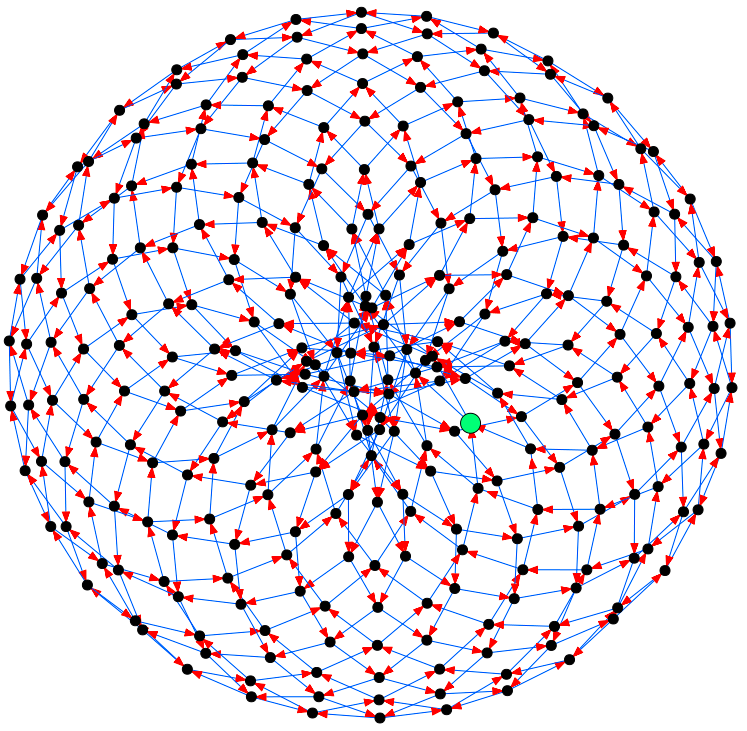
\includegraphics[scale=0.6]{../images/Regular15_NEATO.png}\\[1.0cm]
\end{center}

\begin{center}

% Author and supervisor
\begin{minipage}{0.4\textwidth}
\begin{flushleft} \large
\emph{Authors:}\\
Niels Bj\o rn Bugge Grathwohl\\
Jens Duelund Pallesen
\end{flushleft}
\end{minipage}
\begin{minipage}{0.4\textwidth}
\begin{flushright} \large
\emph{Supervisor:} \\
Jakob Grue Simonsen
\end{flushright}
\end{minipage}
 
\vfill
 
% Bottom of the page
{Department of Computer Science, University of Copenhagen\\
June 2010}
 
\end{center}
 
\end{titlepage}

% Abstract
%!TEX root = ../rapport.tex

\begin{abstract}

This project considers visualization of $\beta$-reduction graphs in the lambda
calculus. We develop a software tool that can take any term in pure lambda
calculus, generate its $\beta$-reduction graph and visualize it with one of
six different graph visualization algorithms. The tool handles reduction
graphs with infinitely many nodes and edges by drawing finite approximations
in which not all redexes have been reduced to their contracta. 

Examples of $\beta$-reduction graphs drawn with the implemented software along
with the lambda terms that generate them are provided. Several families of
terms correspond to well-known classes of graphs, including: $K_n$; the
$n$-dimensional hypercube; the regular, convex $n$-sided polygon and $n$-sided
prisms.

We conjecture that the tool will be useful both for researchers investigating
properties of reduction graphs as well as for students learning about the lambda
calculus.

\end{abstract}


% Table of content
\tableofcontents
\listoffigures

% Chapters
%!TEX root = ../rapport.tex

\chapter{Introduction}

In this work we develop an automatic method for visualization of
$\beta$-reduction graphs of lambda terms. The method has been implemented in
the programming language Python.

Until now, no software for reduction graph visualization existed. Researchers
wanting to visualize reduction graphs have therefore been limited to either
their own drawings or to what they can imagine. Since reduction graphs can be
very large, this posed a very tight constraint on what could be visually
presented.

In our opinion, software for this visualization task presents two primary
challenges: The drawn graphs must be \emph{informative} and
\emph{good-looking}. These two matters are not entirely independent of each
other; very often the particular layout of a graph's two-dimensional embedding
greatly reduces clutter and ``noise'', thus adding information. The opposite
can of course also be the case, which is why the two problems are
interchanged.

The intended user of the software is a theoretical computer scientist that
does research in the field of lambda calculus. Our hope is that researchers
can use this tool to gain new insight into the lambda calculus, and that it
will serve as a source of inspiration for new research because it offers a new
look at a well-known concept.

\section{A Brief History of the Lambda Calculus}

The lambda calculus was developed in the 1930s by Alonzo Church
\cite{Church1932}, contributing to the mathematical search for a foundation
for all mathematics. The attempt was unsuccesful, however, as it was possible
to derive meaningless equations by the Kleene-Rosser paradox
\cite{KleeneRosser1935}. After this setback, Church published a subset of the
theory, known as the \emph{untyped lambda calculus} \cite{Church1936}. This
part of the theory deals only with the concepts relevant for computation, and
does as such not try to lay out a general foundation for all mathematics.
Later on, Church also published a simple, typed version of his theory, known
as the \emph{simply typed lambda calculus} \cite{Church1940} in order to fix
some of the shortcomings of the original calculus. In the present work we deal
with the untyped version, whence the names ``lambda calculus'' and ``untyped
lambda calculus'' will be used as synonyms.

The untyped lambda calculus proved quite useful for computability theory.
Church proposed a definition of the notion ``effectively computable'' using
it, and Turing showed that his ``mechanical'' approach to computability in the
Turing machine is equivalent to Church's approach
\cite{Turing1936,Turing1937}. In the field of programming languages it was
also put to use, as it can be viewed as a Turing-complete programming
language, albeit very cumbersome to use. It is of course not intended to be
used as a ``regular'' programming language, rather, it provides a clean
mathematical framework and notation for language designers to reason about
programming language semantics. For instance, a formal semantics for Algol was
developed by translating the language into lambda calculus and then defining a
semantics for that \cite{Landin1965}.

\section{Expectations of the Reader}

The reader is expected to have a basic knowledge of graphs similar to
``Introduction to Graph Theory'' \cite{Trudeau1994}, along with basic
familiarity with Python similar to ``Python Programming: An Introduction to
Computer Science'' \cite{Zelle2004}. Knowledge of the lambda calculus from e.g.
\cite{Barendregt} Chapter 1, 2 and 3 is an advantage but not a requirement,
since the basic concepts relevant for this work are introduced in a later
chapter.

%!TEX root = ../rapport.tex

\chapter{Preliminaries: Basic Lambda Calculus}
\label{chap:theory}

As a very informal example, here is a function that doubles an integer:
\begin{equation*}
	(\lam{x}{x+x})2=4.
\end{equation*}
This example shows a \emph{bound variable}, $x$, and an implicit \emph{reduction step}. The variable $x$
is said to be bound because the lambda function uses it as an argument. Contrast this to
\begin{equation*}
	(\lam{x}{x+y})2=2+y.
\end{equation*}
Here, $y$ is a variable that has no values assigned to it yet. From
the context we can say nothing about $y$, so we give it the predicate
``free''. In this second example there was yet another reduction step, which 
can be regarded as a rewriting action on the string representing the
lambda term. More informally, one can think of it as ``substituting in''
the values for the bound variables. In the examples above this amounts to
replacing $x$ with the number 2.

% definition af syntax
\section{Syntax}
\begin{definition}
	The lambda calculus consists of \emph{lambda terms} defined over the alphabet:
	\begin{align*}
		x,y,z,\hdots\ &\in V\\
		\lambda\ &\text{ abstractor} \\
		()\ &\text{ parentheses}
	\end{align*}
	where $V$ is the countable, infinite set containing variable names $v_0,v_1,v_2,\hdots$.
	The set of all lambda terms $\Lambda$ is defined inductively as follows:
	\label{def:grammar}
	\begin{align*}
		x\in\Lambda \\
		M\in\Lambda &\Rightarrow (\lam{x}{M})\in\Lambda \\
		M, N\in\Lambda &\Rightarrow (M N)\in\Lambda
	\end{align*}
where $x\in V$.
\end{definition}
\begin{convention}
	A term $\lam{x}{M}$ is called a function.
\end{convention}
\begin{convention}
	For brevity, we leave out the outermost parentheses.
\end{convention}
\begin{convention}\label{con:assoc}
	Evaluation is left associative:
	\begin{equation*}
		M N P \equiv (M N) P
	\end{equation*}
\end{convention}
\begin{convention}\label{con:extent}
	Function bodies extend as far as possible:
	\begin{equation*}
		\lam{x}{M N}\equiv\lam{x}{(M N)}\not\equiv(\lam{x}{M})N
	\end{equation*}
\end{convention}
\begin{convention}
	Functions take exactly one argument, but as syntactic sugar we use:
	\begin{equation*}
		\lam{xy}{xy}\equiv\lam{x}{\lam{y}{xy}}
	\end{equation*}
\end{convention}

\section{Free Variables}

As already indicated, the variables in a lambda term can be divided into
two groups; the free and the bound variables.

\begin{definition}
	The set $FV(M)$ is the smallest set containing all free variables of the lambda
	term $M$, defined by:
	\begin{align*}
		FV(x)&=\{x\} \\
		FV(\lam{x}{M})&= FV(M) - \{x\} \\
		FV(M N) &= FV(M) \cup FV(N)
	\end{align*}
\end{definition}
\begin{definition}\mbox{}
	\begin{enumerate}
		\item If $FV(M)=\emptyset$, $M$ is said to be \emph{closed}.
		\item The set of all closed terms is denoted $\Lambda^0$.
	\end{enumerate}
\end{definition}
\begin{definition}
	A variable $x$ that is not free is \emph{bound}.
\end{definition}

\section{Substitution}

It is possible to substitute
values for free variables. These values are not limited to being just new
variables, but can be any lambda term. A substitution is notated:
\begin{align*}
	M[x:=N]
\end{align*}
with the intuitive meaning that all free occurences of $x$ are replaced with 
the term $N$.
\begin{definition}
Substitution is defined as follows (\cite{Barendregt} 2.1.15):
\begin{align*}
	x[x:=N]&\equiv N \\
	y[x:=N]&\equiv y, \text{ if } x \not\equiv y \\
	(\lam{y}{M})[x:=N]&\equiv\lam{y}{(M[x:=N])}, \text{ if } x\not\equiv y \\
	(\lam{x}{M})[x:=N]&\equiv\lam{x}{M} \\
	(M L)[x:=N]&\equiv(M[x:=N])(L[x:=N])
\end{align*}
\end{definition}
Using this definition, the following result can be shown (\cite{Barendregt} p. 28):
\begin{lemma}\label{lem:subst}\mbox{}
	\begin{enumerate}
		\item $M=M'\Rightarrow M[x:=N]=M'[x:=N]$.
		\item $N=N'\Rightarrow M[x:=N]=M[x:=N']$.
		\item $M=M', N=N'\Rightarrow M[x:=N]=M'[x:=N']$.
	\end{enumerate}
\end{lemma}
Lemma \ref{lem:subst} tells us, informally, that the meaning of a a lambda term
is closed under substitution with equals.

\section{Subterms}

A lambda term $M$ is composed of several parts which we call \emph{subterms}.
\begin{definition}\mbox{}
	\begin{enumerate}
		\item $N\subset M$ denotes that $N$ is a subterm of $M$. The set $Sub(M)$ is the 
		smallest set such that all subterms of $M$ are contained in $Sub(M)$:
		\begin{align*}
			Sub(x) &=\{x\} \\
			Sub(\lam{x}{N}) &= Sub(N) \cup \{\lam{x}{N}\} \\
			Sub(M N) &= Sub(M) \cup Sub(N)  \cup \{M N\} %FIXME det ser da underligt ud?
		\end{align*}
		\item A subterm $N$ of $M$ is called \emph{active} if $N L \subset M$ 
		for a term $L$ and \emph{passive} otherwise.
	\end{enumerate}
\end{definition}
\begin{example}\label{exmpl:subterms}
	The term $M\equiv\lam{x}{xy(\lam{z}{y})}$ has the following subterms:
	\begin{itemize}
		\item $\lam{x}{((xy)(\lam{z}{y}))}\subset M$, passive.
		\item $(xy)(\lam{z}{y})\subset M$, passive.
		\item $xy\subset M$, active.
		\item $\lam{z}{y}\subset M$, passive.
		\item $x\subset M$, active.
		\item $y\subset M$, passive.
	\end{itemize}
\end{example}
Note that the subterm $y$ occurs two times in Example \ref{exmpl:subterms}.

\section{$\alpha$-congruence}

The particular name of a bound variable does not affect the function represented 
by a lambda term. Thus, the two terms
\begin{align*}
	\lam{x}{x} \\
	\lam{y}{y}
\end{align*}
denote the same function, namely the identity. This gives rise to a definition of congruence
that is essential in the lambda calculus.
\begin{definition}\mbox{}
	\begin{enumerate}
		\item For a term $M$, \emph{change of bound variables} is defined as a substitution
		of a part of $M$, $\lam{x}{N}$, with $\lam{y}{N[x:=y]}$, i.e. all occurences of $x$
		are replaced with an occurence of $y$. It is a requirement that $y$ does not 
		occur in $N$.
		\item $M$ and $N$ are $\alpha$-congruent, $M\equiv_\alpha N$, if $N$ is the
		resulting term after a finite sequence of changes of bound variables in $M$.
	\end{enumerate}
\end{definition} 
For instance, we have:
\begin{example}
\begin{align*}
	\lam{x}{x}&\equiv_\alpha\lam{y}{y} \\
	\lam{x}{\lam{y}{xy}}&\equiv_\alpha{\lam{a}{\lam{b}{ab}}} \\
	\lam{x}{\lam{y}{xy}}&\not\equiv_\alpha\lam{y}{\lam{y}{yy}}
\end{align*}
\end{example}
This last example illustrates the need for the requirement that $y$ cannot
occur in $N$. 
\begin{convention}
	\label{con:alpha}
	In the following we will regard $\alpha$-congruent terms as
	being equivalent, so the notation $\equiv$ is used instead of
	$\equiv_\alpha$.
\end{convention}

\section{Contexts}

\begin{definition}\mbox{}
	\begin{enumerate}
		\item A context $C[\ ]$ is an ``unfinished term'' with one hole in it. 
		\item The set $Con$ contains all contexts and is defined as the smallest
		set satisfying these constraints:
		\begin{align*}
			[\ ]&\in Con \\
			M\in\Lambda\Rightarrow M[\ ]&\in Con \\
			M\in\Lambda\Rightarrow [\ ]M&\in Con \\
			C\in Con\Rightarrow \lam{x}{C} &\in Con
		\end{align*}
		\item Terms can be plugged into the holes, thus completing the term. 
		\item When plugging a term into a hole, we do not work modulo 
		$\alpha$-congruence.
	\end{enumerate}
\end{definition}
\begin{example}
	Given the context $C[\ ]\equiv\lam{x}{x[\ ]}$, we can make new lambda terms:
	\begin{align*}
		C[x]&\equiv\lam{x}{xx} \\
		C[\lam{y}{y}]&\equiv\lam{x}{x\lam{y}{y}}
	\end{align*}
\end{example}

\section{$\beta$-reduction}

In this section we shall define a key concept of the lambda calculus which
plays a central role in this report, namely the $\beta$-reduction. This
reduction captures the notion of ``substituting in'' terms for bound variables,
and can be intuitively thought of as ``solving'' a lambda term by reducing it
to a (sometimes) simpler form.

\begin{definition}\label{def:betareduction}\mbox{}
	\begin{enumerate}
		\item \emph{$\beta$-reduction} is a binary relation $\BETA\subseteq\Lambda^2$ such that
		\begin{equation*}
			\BETA=\Big\{\big((\lam{x}{M})N,\ M[x:=N]\big)\big|M,N\in\Lambda\Big\}.
		\end{equation*}
		\item For an element $(M,N)\in\BETA$ we call $M$ a \emph{$\beta$-redex} and
		$N$ a \emph{$\beta$-contractum} of $M$.
		\item A term $M$ is in \emph{$\beta$-normal-form} ($\beta$-nf) if it 
		does not contain any subterms that are $\beta$-redexes.
	\end{enumerate}
\end{definition}
\begin{definition}
	Definition \ref{def:betareduction} is extended to contexts.
	\begin{align*}
		C\big[(\lam{x}{M})N\big]\equiv C\big[M[x:=N]\big]
	\end{align*}
\end{definition}
\begin{definition}\label{def:beta_rel1}
	We have the relations (\cite{Barendregt} def. 3.1.5]):
	\begin{align*}
		(M,N)\in\BETA&\Rightarrow M\barrow N \\
		M\barrow N &\Rightarrow ZM\barrow ZN \\
		M\barrow N &\Rightarrow MZ\barrow NZ \\
		M\barrow N &\Rightarrow \lam{x}{M}\barrow \lam{x}{N} 
	\end{align*}	
\end{definition}
\begin{definition}\label{def:beta_rel2}
	The transitive, reflexive closure of $\barrow$ is notated $\Barrow$:
	\begin{align*}
		M\barrow N &\Rightarrow M\Barrow N \\
		M\Barrow N, N\Barrow L &\Rightarrow M\Barrow L \\
		M\Barrow M & 
	\end{align*}
\end{definition}
\begin{definition}
	The relations from Definitions \ref{def:beta_rel1} and \ref{def:beta_rel2} 
	generate an equivalence relation:
	\begin{align*}
		M\Barrow N &\Rightarrow M=_\beta N \\
		M=_\beta N &\Rightarrow N=_\beta M \\
		M=_\beta N\wedge N=_\beta L&\Rightarrow M=_\beta L
	\end{align*}	
\end{definition}
\begin{definition}
	A term $N$ is a \emph{$\beta$-normal form of $M$} if $M=_\beta N$ and $N$ is in $\beta$-normal form.
\end{definition}
\begin{definition}
	For two terms, $M\Barrow N$, we call $N$ the \emph{reduct} of $M$.
\end{definition}
From these definitions it follows (\cite{Barendregt} 3.1.10), that if $M$ is a
$\beta$-nf then $\neg\exists N:M\barrow N$ and $M\Barrow N\Rightarrow M\equiv N$.

The following example from \cite{Barendregt} p. 52 illustrates the concept:
\begin{example}
	$(\lam{x}{xx})(\lam{y}{y})z\Barrow z$, and hence $(\lam{x}{xx})(\lam{y}{y})z =_\beta z$.
	More elaborately:
\begin{align*}
	(\lam{x}{xx})(\lam{y}{y})z&\barrow(\lam{y}{y})(\lam{y}{y})z \\
	&\barrow(\lam{y}{y})z \\
	&\barrow z
\end{align*}
\end{example}

\section{The Church-Rosser Theorem}

A very important property of the lambda calculus was shown by Church and
Rosser \cite{Church1936}. The following formulations are from
\cite{Barendregt} Chapter 3.

\begin{definition}\mbox{}
	\begin{enumerate}
	\item A binary relation $\rightarrow\subseteq\Delta^2$ satisfies the \emph{diamond property}
	($\rightarrow\models\diamondsuit$) if:
	\begin{align*}
		\forall M,M_1,M_2 : \big(M\rightarrow M_1\wedge M\rightarrow M_2
		\Rightarrow \exists M_3 : \left(M_1\rightarrow M_3 \wedge M_2 \rightarrow M_3\right) \big)
	\end{align*}
	
	\item A relation whose reflexive, transitive closure satisfies the diamond property
	is \emph{Church-Rosser} (CR).
	\end{enumerate}
\end{definition}

A look at Figure \ref{fig:images_diamond} explains why it is called the ``diamond property''.

\begin{figure}[htbp]
	\centering
		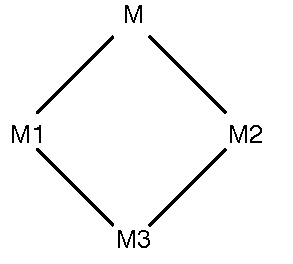
\includegraphics[height=1in]{../images/diamond.pdf}
	\caption[The diamond property.]
	{The diamond property. The lines represent binary relations between the elements.}
	\label{fig:images_diamond}
\end{figure}

\begin{theorem}[Church-Rosser Theorem]\mbox{}
	\begin{enumerate}
		\item The $\beta$-reduction, $\BETA\subseteq\Delta^2$ satisfies the
		diamond property.
		\item The reflexive, transitive closure of the $\beta$-reduction, $\Barrow$, satisfies
		the diamond property. Hence, the $\beta$-reduction is Church-Rosser.
	\end{enumerate}
\end{theorem}

The Church-Rosser theorem implies, informally, that a $\beta$-reduction cannot
get ``stuck'', unless a normal form is being reduced.

\section{Reduction Graphs}

When a $\beta$-redex $M$ contains subterms $\Delta_{0\hdots n}$ that are themselves 
$\beta$-redexes, an ambiguity concerning the order of $\beta$-reductions arises.
Consider the following example from \cite{Barendregt} 3.1.19:
\begin{example}
	Let $M\equiv(\lam{x}{xx})\Delta$ and $\Delta\barrow\Delta'$. We can then perform the two reductions:
\begin{align*}
	M&\barrow(\lam{x}{xx})\Delta' \\
	M&\barrow\Delta\Delta
\end{align*}
\end{example}
The example shows that we can choose to reduce $\Delta$ to its contractum $\Delta'$, or
we can choose to reduce $M$ to its contractum $\Delta\Delta$. This is notated as 
$\overset{\Delta}\barrow$ and $\overset{M}\barrow$ respectively. Different
subterms can have the same contractum, as this example illustrates:
\begin{example}
	Let $\I\equiv\lam{x}{x}$. Then:
\begin{align*}
	\I(\I x)&\overset{\I x}\barrow\I x \\
	\I(\I x)&\overset{\I(\I x)}\barrow\I x
\end{align*}
\end{example}
The set of reductions from a redex $M$ can
be considered as a directed graph, with each arc going out of a node representing
a reduction on some subterm of that node, and each node representing a lambda term that
is the contractum of the terms represented by the nodes parents.
\begin{definition}
	The \emph{$\beta$-reduction graph} of $M$, written $G_\beta(M)$, consists
	of the nodes in the set $V$ and the arcs in the multiset $A$. The set
	of nodes and multiset of arcs in $G_\beta(M)$ are defined as:
	\begin{align*}
		V&=\{N\in\Lambda|M\Barrow N\} \\
		A&=\{(N_0, N_1)\in\Lambda^2|N_0,N_1\in V\wedge N_0\barrow N_1\}
	\end{align*}
	Since $A$ can contain duplicates it follows that if there are more than one
	different reduction step from $N_0$ to $N_1$, that many arcs will be included 
	in $G_\beta(M)$.
\end{definition}

\begin{example}\mbox{}
	\begin{enumerate}
		\item The reduction graph illustrated in Figure \ref{fig:images_graphs_graf2}
		for the term $\I x$, $G_\beta(\I x)$, with
		the previous definition of $\I$ captures the reduction $\I x\barrow x$.
		
		\item $G_\beta(\I(\I x))$ is illustrated in Figure \ref{fig:images_graphs_graf1}.
		
		\item Let $\Omega\equiv(\lam{x}{xx})(\lam{x}{xx})$. $G_\beta(\Omega)$
		can be seen in Figure \ref{fig:images_graphs_graf3_omega}.
		
		\item Let $\W\equiv\lam{xy}{xyy}$. $G_\beta(\W\W\W)$ is illustrated in
		Figure \ref{fig:images_graphs_graf4_www}.
		
		\item Let $M\equiv\lam{x}{(\lam{y}{yy})x}$. $G_\beta(MM)$ is pictured in
		Figure \ref{fig:images_graphs_graf5_MM}.
		
		\item Let $w_3\equiv\lam{x}{xxx}$. Figure \ref{fig:images_graphs_graf6_w3w3}
		contains the reduction graph. Note that this graph contains an infinite 
		amount of nodes and arcs.
		
		\item In Figure \ref{fig:images_graphs_graf7_omega_w3} there is another
		example of a graph containing an infinite amount of nodes and arcs. This
		graph captures qualities found in the two graphs $G_\beta(\Omega)$ and
		$G_\beta(w_3w_3)$.
	\end{enumerate}
	Note that these examples only serve to illustrate the \emph{structure} of a 
	$\beta$-reduction graph, not the actual graph visualization that we develop
	in this paper.
	\begin{figure}[htbp]
		\centering
		\begin{tabular}{ccc}
			\subfigure[$G_\beta(\I x)$]{
				
\includegraphics{../images/graphs/graf2.pdf}
				\label{fig:images_graphs_graf2}
			} &
			\subfigure[$G_\beta(\I(\I x))$]{
				
\includegraphics{../images/graphs/graf1.pdf}
				\label{fig:images_graphs_graf1}
			} & 
			\subfigure[$G_\beta(\Omega)$]{
				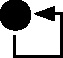
\includegraphics{../images/graphs/graf3_omega.pdf}
				\label{fig:images_graphs_graf3_omega}
			} \\ \\
			\subfigure[$G_\beta(\W\W\W)$]{
				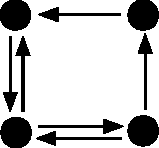
\includegraphics{../images/graphs/graf4_www.pdf}
				\label{fig:images_graphs_graf4_www}
			} \hspace{1.5em}
			&
			\subfigure[$G_\beta(MM)$]{
				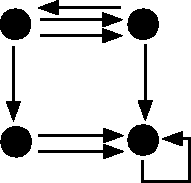
\includegraphics{../images/graphs/graf5_MM.pdf}
				\label{fig:images_graphs_graf5_MM}
			}\hspace{1.5em}
			&
			\subfigure[$G_\beta(w_3w_3)$]{
				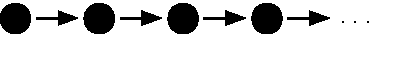
\includegraphics{../images/graphs/graf6_w3w3.pdf}
				\label{fig:images_graphs_graf6_w3w3}
			}
		\end{tabular}
		\caption
		[Examples of $\beta$-reduction graphs for different lambda terms.]
		{Examples of $\beta$-reduction graphs for different lambda terms. 
		Taken from \cite{Barendregt}.}
	\end{figure}
	\begin{figure}[htbp]
		\centering
			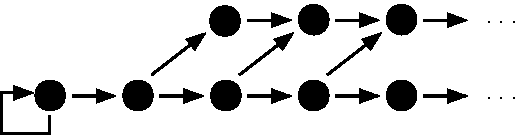
\includegraphics{../images/graphs/graf7_omega_w3.pdf}
		\caption{The $\beta$-reduction graph $G_\beta(\Omega w_3)$}
		\label{fig:images_graphs_graf7_omega_w3}
	\end{figure}
\end{example}

Not all directed graphs are reduction graphs. Because of the Church-Rosser
property, reduction graphs like the ones pictured in Figure
\ref{fig:images_graphs_impossible} cannot exist for any lambda term. Any graph
with more than two nodes with an in-degree of 1 cannot be a reduction graph in
the lambda calculus because of this property. In \cite{VenturiniZilli1984251}
are more thorough discussion of what cannot be a reduction graph is presentd.

\begin{figure}[htbp]
	\centering
	\subfigure[The diamond property is obviously violated in this graph.]{
		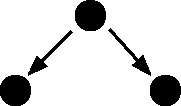
\includegraphics{../images/graphs/impossible1.pdf}
	}
	\subfigure[It is too in this graph; no less than three normal forms
	should be produced in order to make this graph.]{
		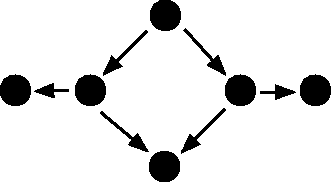
\includegraphics{../images/graphs/impossible2.pdf}
	}
	
	\caption{Examples of directed graphs that cannot be reduction graphs.}
	\label{fig:images_graphs_impossible}
\end{figure}

%!TEX root = ../rapport.tex

\chapter{Existing Visualizations of the $\lambda$-Calculus}

In this chapter we will discuss what already exists in areas related to this
work. We give a small survey of software that can visualize some aspect of the
lambda calculus, as well as work discussing properties of the reduction
graphs.

We have not in our research found anything exactly similar to what we are
trying to do. There do exist many examples where a given reduction has been
visualized, but never in a way giving a complete insight into the evaluation
of the lambda term. We have been able to find 9 examples of previous work
related to our work, and in the following section we will focus on two of
them:
\begin{itemize}
	\item In \cite{Citrin+Hall+Zorn+1995a}, a visual notation for lambda terms 
	is developed, wherein one uses circles inside other circles to represent
	what is normally written with $\lambda$-symbols and variable names.
	
	\item A theoretical discussion of reduction graphs and some of their properties
	can be found in \cite{VenturiniZilli1984251,297368}. 
	
	\item In \cite{Sestoft96standardml} a tool called a \emph{lambda reducer} is 
	presented as an example application. It visualizes different reduction 
	strategies in a web-based interface.
	
	\item The authors of \cite{DBLP:journals/entcs/RuizV09} present a program
	that draws a parse-tree-like representation of lambda terms that the user can interact
	with. 
	
	\item The ``Animated Lambda Calculus Evaluator'' from \cite{AnimatedLambdaCalculusEvaluator}
	is another parse-tree-like drawing of lambda terms.
	
	\item The ``Lambda Animator'' \cite{lambdaAnimatorThyer} and ``Alligator Eggs'' \cite{Alligator}
	are presented more in-depth below.
	
\end{itemize}

The present work differentiates itself from all of the above, since we are
trying to visualize \emph{reduction graphs}, whereas all the mentioned visualizers
are build to draw specific \emph{lambda terms} in some way, for instance as a syntax
tree.

\section{Alligator Eggs -- A Puzzle Game by Bret Victor}

The ``Alligator Eggs - A Puzzle Game'' \cite{Alligator} is a ``fun'' and
children-like way of visualizing $\beta$-reductions of a lambda term. It was
originally not intended to be a computer program; the author instead designed
a set of drawings meant to be printed and cut out. This way, the visualization
can be used as a game. It visualizes the syntactic structure of lambda
terms, and the allowed ``moves'' in the game correspond to $\alpha$-conversion or
$\beta$-reduction.

The game uses a simple graphical alphabet:
\begin{description}
	\item[A hungry alligator] represents a lambda abstraction. The symbol can
	have different colors, analogously to variable names in ordinary lambda calculus.
	\item[An old alligator] is a parenthesis. It can only be white.
	\item[An egg] is a variable. It, too, can take on different colors.
\end{description}
Alligators are organized vertically into ``families''. The different families
are organized horizontally next to each other, and they are guarded by either an
old or a hungry alligator. The old alligator only concerns itself with
guarding, while the hungry alligator also has one or more eggs associated. If
an alligator and an egg are associated with each other, they have the same
color. It is straightforward to see the analogy to lambda terms.

With this alphabet, the rules are defined as follows:
\begin{description}
	\item[The Eating Rule] states, that the topmost hungry alligator of a family can
	eat the family in front of it. When it does this it dies, but the eaten family
	is resurrected in its entirety from all the eggs associated with the hungry, dead
	alligator. This rule corresponds to a $\beta$-reduction. 
	\item[The Color Rule] states, that if an eaten family contains alligators and eggs
	in the same color as some alligators or eggs in the eating family, these must change colors
	to some new, unused color. This rule corresponds to an $\alpha$-conversion.
	\item[The Old Age Rule] states, that if the topmost alligator of a family is
	an old alligator, this alligator may die and nothing will happen. This is in analogy
	to the convention, that outermost parentheses in lambda terms are removed.
\end{description}

In Figure \ref{fig:images_alligatorEat} we see the Eating Rule in use. The
green alligator will eat whatever is in front of it. In this case it will eat
the yellow alligator and its yellow egg. After the green alligator has eaten
the yellow alligator and egg, it will die and its egg will hatch into what it
has eaten. ``The miracle of life'', as the author calls it. This so-called
``miracle'' is in our profane terminology called a $\beta$-reduction, as
mentioned above.

\begin{figure}[htbp]
	\centering
		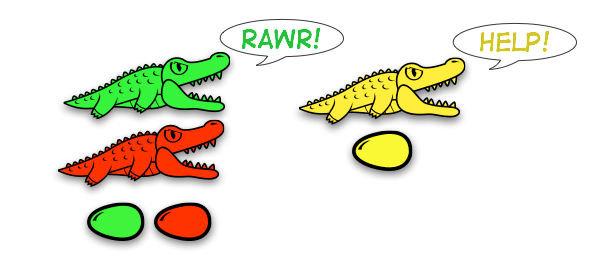
\includegraphics[width=2in]{../images/alligatorEat.png}
	\caption{A reduction visualized as an alligator eating}
	\label{fig:images_alligatorEat}
\end{figure}

In Figure \ref{fig:images_alligatorOld} we see an example of the old age rule.
In Figure \ref{fig:images_alligatorOld} (a) the old alligator guards more than
one alligator and therefore works as a parenthesis. Now the green alligator
eats the red alligator. We now see in Figure \ref{fig:images_alligatorOld} (b)
that the old alligator only has the red alligator to guard, which is the
reason for that it will now die. In normal mathematical words, this means that
the parenthesis only concludes one element and is therefore useless. Figure
\ref{fig:images_alligatorOld} (c) shows the end result with the old alligator
dead.

\begin{figure}[htbp]
	\centering
		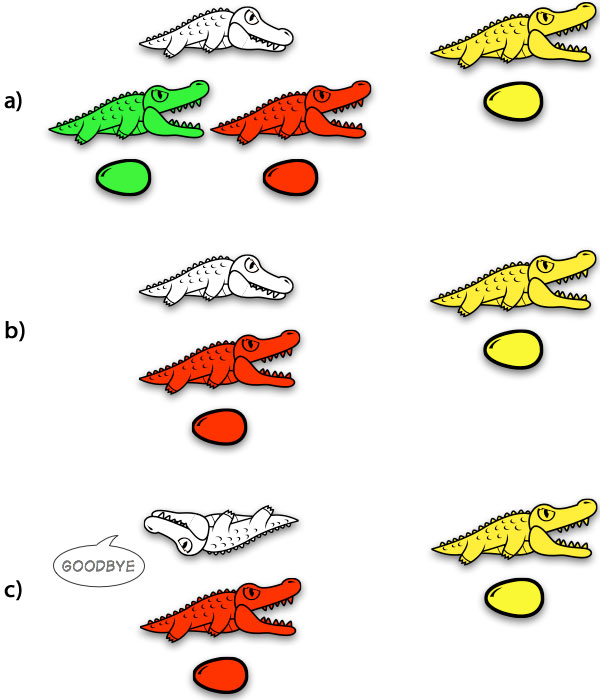
\includegraphics[width=2in]{../images/alligatorOld.jpg}
	\caption{Example of the old age rule}
	\label{fig:images_alligatorOld}
\end{figure}

``Alligator Eggs - A Puzzle Game'' does not deal with the same kind of
visualization tasks that we do in this project. It basically presents a
creative way of drawing syntax trees and a new, carnivorous terminology for
the transformations in the lambda calculus. 

The game has been implemented as a Java program, so that one does not need to
actually print out the alligators \cite{AlligatorTool}.

\section{Lambda Animator by Mike Thyer}

The ``Lambda Animator'' is a representation of lambda terms in syntax tree form. It
is implemented in Java and available online via a Java Applet
\cite{lambdaAnimatorThyer}.

\begin{figure}[!htbp]
	\centering
		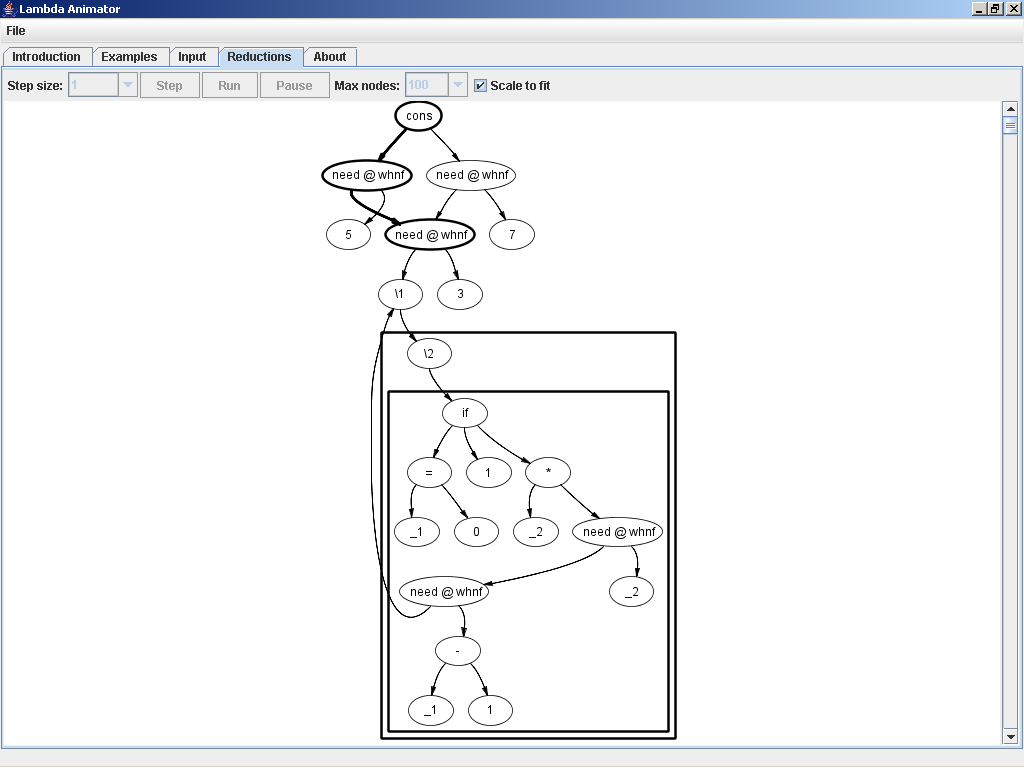
\includegraphics[scale=0.1]{../images/lambdaAnimator.png}
	\caption{Screenshot of the Lambda Animator tool}
	\label{fig:images_lambdaAnimator}
\end{figure}

The Animator does not seem very smooth and does not produce graphs that are
neither pretty nor especially visually informative, since they can be very
large. The implementation in the form of a Java applet does have some
advantages in terms of easy access to the tool, though.

It can give an reasonable overview when the lambda terms are not too complex.
In Figure \ref{fig:images_lambdaAnimatorReduction} there is an example of a
simple $\beta$-reduction. Note that the lambda calculus used in the Animator
has syntactic sugar in the form of function names etc.

\begin{figure}[!htbp]
	\centering
		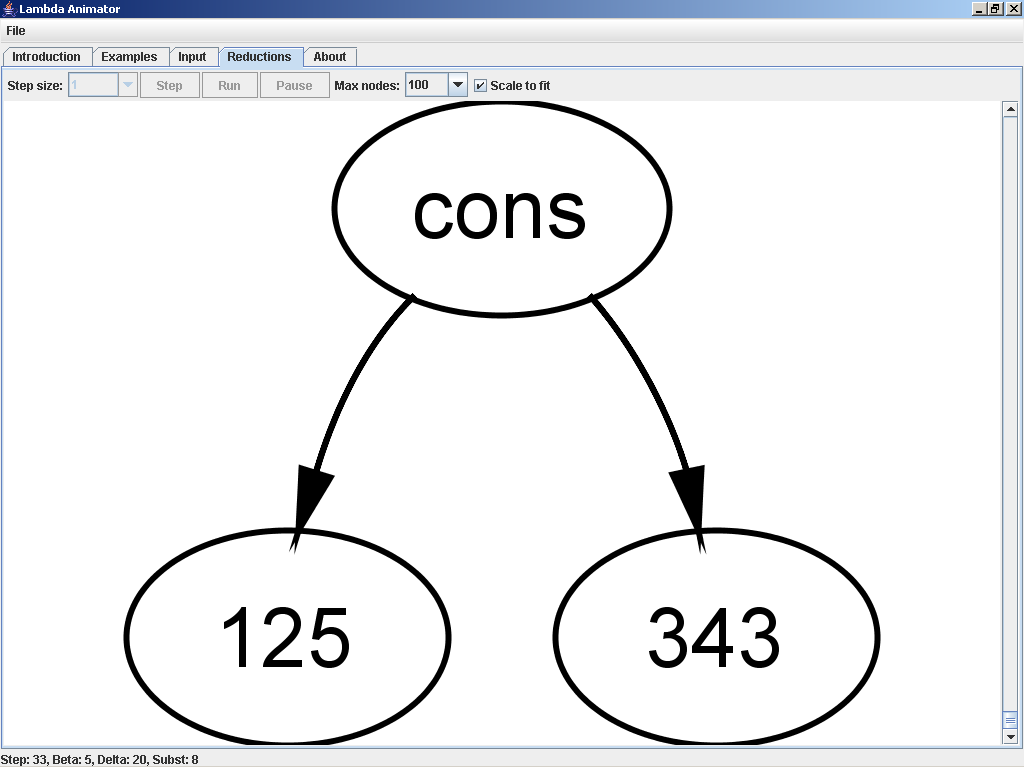
\includegraphics[scale=0.25]{../images/lambdaAnimatorReduction.png}
	\caption{Example of a simple $\beta$-reduction in the Lambda Animator}
	\label{fig:images_lambdaAnimatorReduction}
\end{figure}

\begin{figure}[!htbp]
	\centering
		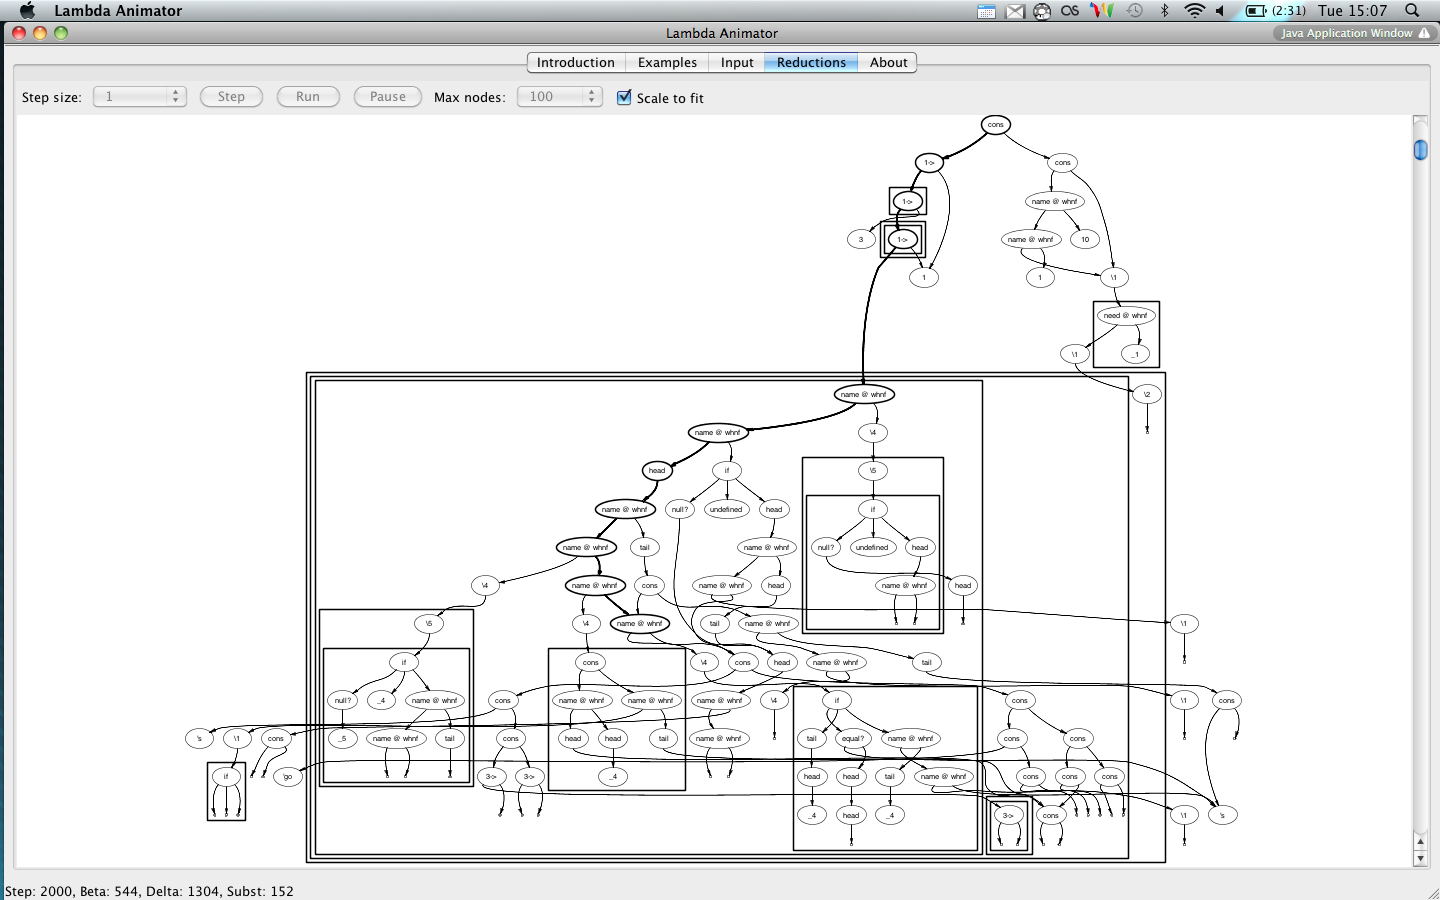
\includegraphics[scale=0.25]{../images/lambdaAnimatorComplex.png}
	\caption{Complex example in the Lambda Animator}
	\label{fig:images_lambdaAnimatorComplex}
\end{figure}

When dealing with more complex lambda terms it easily gets chaotic. In Figure
\ref{fig:images_lambdaAnimatorComplex} there is another example, in which one
can see that the informativeness seems to drastically degrade when the term
complexity is increasing.



%!TEX root = ../rapport.tex

\chapter{Graph Drawing}\label{chap:graph_drawing}

A \emph{graph drawing} is an embedding of the abstract, mathematical concept
of a graph on a two-dimensional surface. A \emph{graphic standard} is the
translation between the abstract graph and graphic symbols representing the
graph. Different graphic standards exist, but the most common ones represent
vertices by dots or filled circles and edges $(u,v)$ by curves connecting the
symbols representing $u$ and $v$. In this chapter we will briefly summarize
the different, relevant graphic standards and methods for drawing them.

Battista et al. give a more thorough overview of the literature in several
different areas of research related to graph drawing in \cite{DiBattista1994}.

\section{Aesthetics}

Graph drawing was motivated by the need for conveying information embedded in
graphs to humans, for instance in the fields of VLSI circuit design, social
network analysis and algorithm visualization. Thus, the quality of a graph
drawing depends heavily on its ability to clearly convey its information,
making it easy for the reader to decipher it. Different \emph{aesthetic
measures} have therefore been developed, depending on the type of information
that the graph must deliver. Common aesthetics are \cite{DiBattista1994}:
\begin{itemize}
	\item The distance between adjacent nodes is
	sought to be minimized, since it can be difficult to get an overview of the
	drawing if edges tend to be very long.
	
	\item The area covered by the graph -- the minimum bounding box of the 
	graph -- can also be an important factor, especially if the drawing is 
	supposed to be in print.
	
	\item When a lot of edges in the graph cross, the informativeness of the 
	graph rapidly deteriorates. Therefore it is desirable to minimize the 
	number of crossing edges in the drawing. In general, it is impossible to 
	remove all crossing edges.
	
	\item If the data contains symmetries we naturally want those to be
	represented as graphical symmetries too.
	
	\item Edges should contain as few bends as possible.
	
	\item Edges should have uniform length.
	
	\item The vertices must be distributed uniformly on the graphic.
\end{itemize}
Studies of graph drawing aesthetics are presented in
\cite{Purchase1997,Purchase2001,Purchase2010}. They indicate that the most
important aesthetic measure is the number of edge crossings.

Most often, graph aesthetics are ``competitive'' so that optimality of one
aesthetic measure means suboptimality of another. Aesthetic measures can be
regarded as optimization goals for graph drawing algorithms. They are in
general NP-hard, so heuristic approaches are used
\cite{Johnson1982,Johnson1984,Garey1983}.

\section{Planarity Issues}

The graphs that can be drawn without any crossing edges are called
\emph{planar graphs}. Not all graphs are planar, a famous example being $K_5$
-- the complete graph with five vertices (Figure \ref{fig:images_graphs_k5}).
There exist many algorithms that draw planar graphs, so to draw a non-planar
graph it is common to start with making the graph planar, a process known as
\emph{planarization}, and then draw the planar version. Afterwards, the
drawing can be altered such that it represents the original non-planar graph.

\begin{figure}[htp]
	\centering
	\begin{tabular}{cc}
		\subfigure[$K_4$.]{
			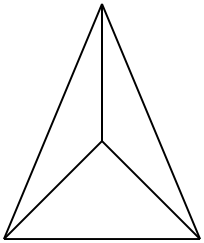
\includegraphics[height=1.3in]{../images/graphs/k4.png}
			\label{fig:images_graphs_k4}
		}\hspace{1.5em}
		&
		\subfigure[$K_5$.]{
			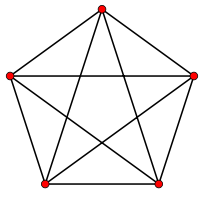
\includegraphics[height=1.3in]{../images/graphs/k5.png}
			\label{fig:images_graphs_k5}
		}		
	\end{tabular}
	\caption
	[$K_4$ and $K_5$.]
	{Examples of a planar and a non-planar graph; the complete graph
	with 4 and 5 nodes, respectively.}
\end{figure}

There exist different methods for planarization. Cai et al. present an
$O(m\log n)$-time algorithm for finding the \emph{maximal planar subgraph}
\cite{Cai1993}. One can also try to find the drawing with the minimum number
of edge crossings. This problem is NP-hard as shown in \cite{Garey1983}, but
heuristics for minimizing the number of crossings are given in
\cite{Ferrari1969}. Another planarization technique is called
\emph{splitting}. A splitting operation converts a node $v$ to two nodes $v_1$
and $v_2$, attaching the neightbours of $v$ to either $v_1$ or $v_2$.
Heuristics for planarization by splitting are discussed in \cite{Eades1993}. 

\section{Planar Representations}

A \emph{planar representation} is a data structure that represents possible
planar embeddings of graph, i.e. which combinations of node positions give
rise to a planar graph. Many drawing algorithms construct a drawing from a
planar representation -- first by testing for planarity, then contructing a
planar representation and then use a drawing algorithm to draw this
representation.

A \emph{path addition} approach to planarity testing was presented by Hopcroft
\cite{Hopcroft1974,Deo1976}. Another approach called the \emph{vertex
addition} approach is presented in \cite{Booth1976}. Both of these methods for
planarity testing run in linear time. Chiba et al. modified the methods of
\cite{Booth1976} to construct planar representations \cite{Chiba1985}.

\section{Straight-line Drawing}

For an undirected graph, the graphic standard with all edges represented by
straight lines is called a \emph{straight-line drawing}. Eades presented an
approach to straight-line drawing using a spring-metaphor
\cite{Eades1984,Fruchterman1991}. In this system, vertices are regarded as
rings and edges are regarded as springs. The springs attract the rings if they
are too far apart and repel them if they are too close. This category of
drawing algorithms is called ``force-directed'' algorithms.

In \cite{Lipton1985} the authors present an approach that focus mainly on
capturing symmetries in the graphs. However, this approach is computationally
very expensive when compared to \cite{Eades1984}.

Another approach is to associate an energy function to a drawing, representing
the ``quality'' of the drawing with respect to the chosen aesthetic measures
by an amount of energy, and then use simulated annealing to compute the
two-dimensional graph embedding \cite{Davidson1996}.

A mixture of different techniques is presented by Tunkelang in
\cite{Tunkelang1992} that focus on computing the aesthetic cost of a drawing,
the order of node placement and local optimization techniques.

It was shown early that every planar graph can be drawn as a planar
straight-line drawing \cite{Wagner1936,Fary1948,Stein1951}. Tutte studied
\emph{convex drawings} of planar graphs, which is a drawing where the faces
consisting of the graph edges are all convex polygons \cite{Tutte1960} (Figure
\ref{fig:images_graphs_convex_1}). Thomassen furthermore characterized the
class of graphs that can be embedded in a convex drawing \cite{Thomassen1980},
and Chiba et al. give a linear time algorithm for making convex drawings using
Thomassen's results \cite{Chiba1984}.
\begin{figure}[htp]
	\centering
		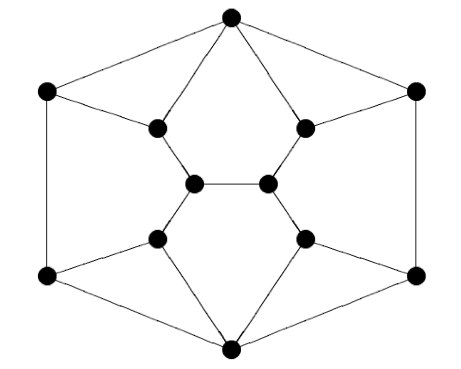
\includegraphics[height=1.5in]{../images/graphs/convex_1.png}
	\caption
	[A convex drawing of a graph.]
	{A convex drawing of a graph. All faces are drawn as convex 
	polygons. (Taken from \cite{DiBattista1994}, Figure 8.)}
	\label{fig:images_graphs_convex_1}
\end{figure}

An aesthetic measure for straight-line drawings is the total edge length.
Becker et al. show that the there is a unique and convex optimal straight-line
drawing with the external face a prescribed convex polygon \cite{Becker1987}.
On the other hand, constructing a planar straight-line drawing with a
prescribed edge length, as measured by the Euclidean metric, is NP-hard
\cite{Eades1990}. 

The performance of several drawing algorthms are compared in \cite{Jones1991}.
The quality of the drawings is measured in terms of the standard deviation of
angle size between edges, the edge length and the face area.

\section{Orthogonal Grid Drawing}

The graphic standard where all edges are either parallel or orthogonal and
fixed to a grid is called \emph{orthogonal grid drawing}, see Figure
\ref{fig:images_graphs_orthogonal_1}. This type of drawing was originally
motivated by circuit layout problems. A common aesthetic measure for this type
of graph is the amount of bends on edges, as well as the area that the drawing
covers. These aesthetics not only affect readability; in circuit design they
have a direct impact on the quality of the circuit that is produced.

In \cite{Batini1984,Tamassia1988} the authors present a general method for the
construction of orthogonal grid drawings. It can be subdivided into three
steps: first the graph is planarized, then an orthogonal shape is computed
based on the planarized graph, and finally this shape is made as compact as
possible to produce the final drawing. This general approch allows orthogonal
grid drawings of many different types of graphs.

It is an NP-complete problem to determine whether a graph can be embedded in a
planar orthogonal drawing without bends, whence the bend-minimization problem
is NP-hard \cite{Garg1994}.

\begin{figure}[htp]
	\centering
		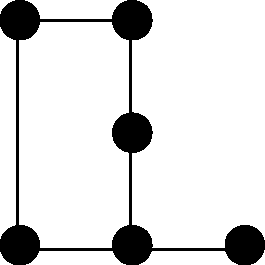
\includegraphics[height=1in]{../images/graphs/orthogonal_1.pdf}
	\caption{An orthogonal grid drawing of a graph.}
	\label{fig:images_graphs_orthogonal_1}
\end{figure}

\section{Visibility Representations}

In a \emph{visibility representation}, each vertex is represented as a
horizontal line and each edge as a vertical line. The vertical lines intersect
exactly those horizontal lines that the corresponding edges connect
\cite{Duchet1983}, see Figure \ref{fig:images_graphs_visibility_repr_1}.
Visibility representations were originally motivated by VLSI layout because it
gives regular, modular graphs \cite{Schlag1985}.

An overview of different classes of visibility representations and linear time
drawing algorithms is given by Tamassia et al. \cite{Tamassia1986}. Often the
first step in creating a visibility representation of an undirected graph is
to create a \emph{bipolar orientation} of it. A bipolar orientation of an
undirected graph is an orientation of the edges of the graph such that the
resulting \emph{directed} graph is acyclic and has excatly one source -- a
vertex having only outgoing edges -- and exactly one sink -- a vertex with
only incoming edges. Properties of bipolar orientations are investigated in
\cite{Fraysseix1993}.

\begin{figure}[htp]
	\centering
	\subfigure{
		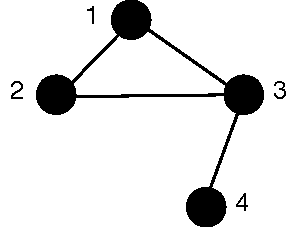
\includegraphics[height=1in]{../images/graphs/visibility_repr_1.pdf}
	}
	\subfigure{
		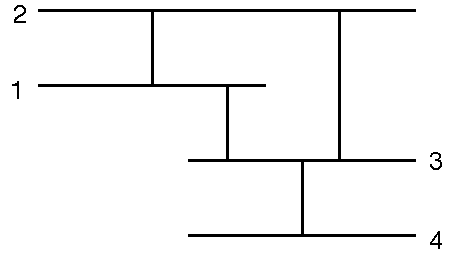
\includegraphics[height=1in]{../images/graphs/visibility_repr_2.pdf}
	}
	\caption{A graph $G$ and its visibility representation.}
	\label{fig:images_graphs_visibility_repr_1}
\end{figure}


\section{Miscellaneous Graphic Standards}

Ozawa proposes a graphic standard where all vertices are dots on a straight
line, and edges are drawn as half-circles over or under the line
\cite{Ozawa1980}, as exemplified in Figure \ref{fig:images_graphs_circles_1}.
\begin{figure}[htp]
	\centering
		
\includegraphics[height=0.6in]{../images/graphs/circles_1.pdf}
	\caption
	[The approach suggested by Ozawa.]
	{The approach suggested by Ozawa \cite{Ozawa1980}.}
	\label{fig:images_graphs_circles_1}
\end{figure}

For cubic graphs that are planar, Kant proposes a method for placing them on a
hexagonal grid in linear time \cite{Kant1992}.

Problems in architectural design motivated a graphic standard where vertices
are represented by polygons and an edge between two vertices are represented
as the two corresponding polygons being geometrically adjacent
\cite{Bhasker1988}. A variant of this graphic standard is the
\emph{tessellation representation} in which vertices, edges and faces of a
planar embedding of a graph is represented as rectangles, and adjacencies
between rectangles correspond to incidencies in the graph \cite{Tamassia1989}
-- see Figure \ref{fig:images_graphs_tessellation}.

\begin{figure}[htp]
	\centering
	\subfigure{
		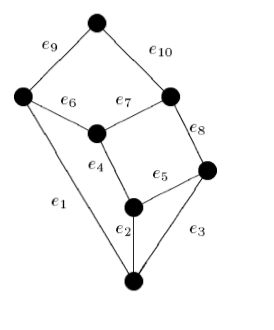
\includegraphics[height=2in]{../images/graphs/tessellation_1.png}
	}
	\subfigure{
		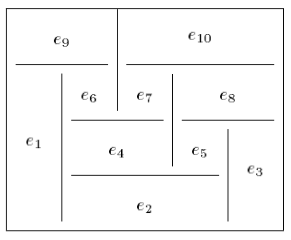
\includegraphics[height=2in]{../images/graphs/tessellation_2.png}
	}
	\caption
	[A tessellation representation of a graph.]
	{A tessellation representation of a graph. (Taken from \cite{DiBattista1994}, Figure 11.)}
	\label{fig:images_graphs_tessellation}
\end{figure}

Dickerson et al. present the graphic standard \emph{confluent drawing} along
with heuristics for it \cite{Dickerson2005} -- see Figure
\ref{fig:images_graphs_confluent}. In this approach, groups of edges are
merged together to what the authors call ``tracks'', and the graph can then be
drawn without crossing edges.

\begin{figure}[htp]
	\centering
	\subfigure{
		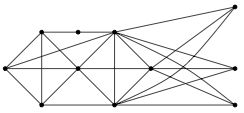
\includegraphics[height=1in]{../images/graphs/confluent_1.png}
	}
	\subfigure{
		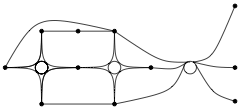
\includegraphics[height=1in]{../images/graphs/confluent_2.png}
	}
	\caption
	[A non-confluent and a confluent drawing of the same graph.]
	{A non-confluent and a confluent drawing of the same graph. 
	(Taken from \cite{Dickerson2005}, Figure 5.)}
	\label{fig:images_graphs_confluent}
\end{figure}

\section{Directed Graphs}

Directed acyclic graphs are used to represent hierachical structure, for
instance in dependency graphs. It is desirable to draw these graphs such that
all edges point in the same direction. A drawing is called \emph{upward} if
all edges are pointing upwards. 

For directed graphs there exists the notion of \emph{upward planarity}, which
corresponds to the notion of planarity for undirected graphs. A graph is
upward planar if it can be drawn without any crossing edges and with all edges
pointing upwards. Algorithms for drawing upward planar graphs are given in
\cite{DiBattista1988}. 

A drawing that is upward planar and in which all edges are straight lines is
called a \emph{Hasse diagram}. These drawings are commonly used to represent
partially ordered sets, and a drawing algorithm is given in
\cite{Jurgensen1983}. Thomassen characterizes the graphs that have a Hasse
diagram in \cite{Thomassen1989}. 

When drawing a directed acyclic graph, three steps corresponding to the case
with an undirected graph are used: the graph is upwards planarized, a planar
representation is found and this representation is drawn with a drawing
algorithm. It is an NP-complete problem to test whether a graph is upward
planar in general \cite{Garg1994}, but polynomial time algorithms exist for
special cases, among others in \cite{DiBattista1990}. A survey of efficient
algorithms that take a planar representation and draw the graph is given in
\cite{Tamassia1990}.

If all vertices are placed on a set of straight, equally spaced lines, with
edges going only between vertices on different lines and not overlapping, the
drawing is said to be a \emph{hierachical drawing}. The procedure for making a
hierachical drawing has three steps: assign vertices to the different lines
such that all edges point upwards, find a permutation of the vertices in which
no edges overlap and finally tune the positions of the vertices to minimize
the number of edge bends. A comprehensive approach is presented by Sugiyama
et al. \cite{Sugiyama1981}. The algorithms used at the three steps are
analysed in \cite{Lin1992}.

For a directed graph that contains cycles it is often desirable to represent
the \emph{flow} of the graph. This is done by maximising the number of edges
that point upwards, which is equivalent to finding the minimum number of edges
that need to be reversed in order to make the graph acyclic. This problem is
in general NP-complete, but there exist polynomial time algorithms for special
cases \cite{Frank1981}. Heuristics for the problem are discussed in
\cite{Berger1990}. After making a graph acyclic, the techniques previously
mentioned can be used. If the representation of flow in the graph is not
important, the acyclic techniques can be applied directly, ignoring the edge
directions.

\section{Issues Related to Large Graphs}

When the size of the graph to be drawn becomes sufficiently large, a host of
new issues appears. First of all there is the question about performance;
several algorithms discussed above and in the referenced papers would be
unacceptably slow if applied to a graph with e.g. $10^4$ nodes and
$3\cdot10^4$ edges. It can therefore sometimes be necessary to alter the
methods. Furthermore there is the problem of room -- there simply has to be
enough room on the monitor for the drawing to fit. In this section we will
briefly discuss a few such methods. A more rigorous study can be found in
\cite{Herman2000}.

For a large graph with $10^4$ nodes and $3\cdot10^4$ edges, the probability
that the graph is planar is very small, and since a planarity check on such a
graph will be slow it is usually just skipped. 


Since a lot of applications of graph drawing techniques operate with large
graphs that cannot be placed all at once on a normal computer monitor, methods
to single out special parts of the drawing and only show these have been
developed. Since one will usually be interested in the whole graph, or at
least most of it, navigational methods have also been studied. 

One method to solve the problem of showing a huge drawing on a relatively
small monitor is to use a ``fisheye'' effect. This effect functions as a
``magnifying glass'' that highlights, or enlarges, the area of the graph
currently in focus while at the same time minimizing the other parts. Using
this, a user can navigate and study a large graph that would otherwise be
drawn with node and edge representations too small for the human eye to
discern. The method utilizes a distortion function, $d:[0,1]\mapsto[0,1]$,
that monotonically maps the interval $[0,1]$ to itself. Figure
\ref{fig:images_fisheye_distortion} shows an example of two distortion functions
as well as an illustration of the effects on a plane.
\begin{figure}[htp]
	\centering
	\subfigure{
		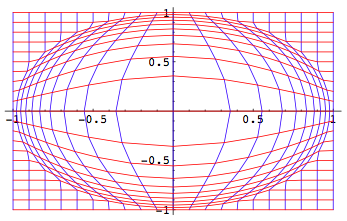
\includegraphics[height=1.7in]{../images/fisheye_distortion.png}
	}
	\subfigure{
		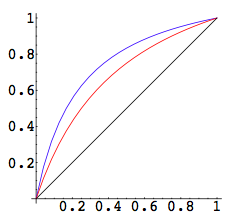
\includegraphics[height=1.9in]{../images/fisheye_distortion_func.png}
	}
	\caption
	[Distortion of a regular grid and a distortion function.]
	{Distortion of a regular grid along with an example of a distortion function. The blue and
	red line represent two different distortion functions, and the black line is 
	the ``normal'', non-distorted view. 
	(Taken from \cite{Herman2000}, Figure 17 and 18.)}
	\label{fig:images_fisheye_distortion}
\end{figure}

A related method is to draw the graph in a hyperbolic coordinate system
instead of an Euclidean. This gives the impression that the graph is drawn on
a sphere, where the graph elements lying on the part of the sphere pointing
towards the observer appear to be enlarged. If this sphere can be rotated by
the user, she can decide which parts of the graph to enlarge and which not,
analogously to the fisheye effect.

If a graph drawing algorithm can reduce the amount of elements, large-scale
structures can be represented in a comprehensible fashion, even though the
underlying graph may contain too many nodes for a normal drawing method. This
approach is called \emph{clustering}. The essence of the method is to find
groups, or clusters, in the graph that have something in common and then draw
the graph consisting of the clusters instead of the original graph. If the
clustering algorithm is chosen properly, structures in graphs otherwise
seemingly chaotic can be easily discerned. One challenging part of the
approach is to find a sensible balance between number of clusters and number
of nodes per cluster, as well as devising a fitting similarity measure for the
clustering algorithm. 

% Relatedly, methods that can intelligently hide parts of the graph deemed
% non-interesting can also greatly increase the clarity of the drawing. 

% clustering
% hiding
% no planarity check/solution
% incremental exploration
% focus+context (hyperbolic, fisheye etc.)
% navigation



% G. Di Battista, P. Eades, R. Tamassia, and I. G. Tollis, 
%   Graph Drawing, Prentice Hall, Upper Saddle River, NJ, 1999.

% Pilehoveder?


%!TEX root = ../rapport.tex

\chapter{Properties of $\beta$-reduction Graphs}

The preceding discussion of graph drawing concerns the problem of drawing
\emph{general} graphs. However, we focus not on general but on one specific
kind of graph: the $\beta$-reduction graph. It is important to identify the
most important characteristics of this graph type in order to be able to
choose relevant and meaningful drawing methods. Also, identifying the
properties that we actually want to highlight is relevant both for the
implementation of the functions that generate the reduction graphs as well as
for the functions that issue the actual drawing commands.

\section{Size}

Reduction graphs vary greatly in size, from one node to an infinite amount of
nodes and edges. For example, $G_\beta(\lam{x}{x})$ contains one node and zero
edges since there are no reducts in the term. On the other hand, the graph
$G_\beta((\lam{x}{xxx})(\lam{x}{xxx}))$ contains infinitely many nodes and
edges. 

In Figure \ref{fig:images_inf_reduction_graph} there are two different
drawings of (a part of) the graph $G_\beta((\lam{a}{b}) (\lam{x}{(xxx)}
\lam{y}{(yyy)}))$. This graph has infinitely many edges and nodes, so the
structure seen in the Figure will continue to grow. 

The layout algorithms are presented in Chapter \ref{chap:implementation}.

\fact
$\beta$-reduction graphs can have an infinite amount of nodes and edges.
\begin{figure}[htpb]
	% #a.(b) (#x.((x x) x) #y.((y y) y))
	\centering
	\subfigure[Drawn using the Circo algorithm.]{
		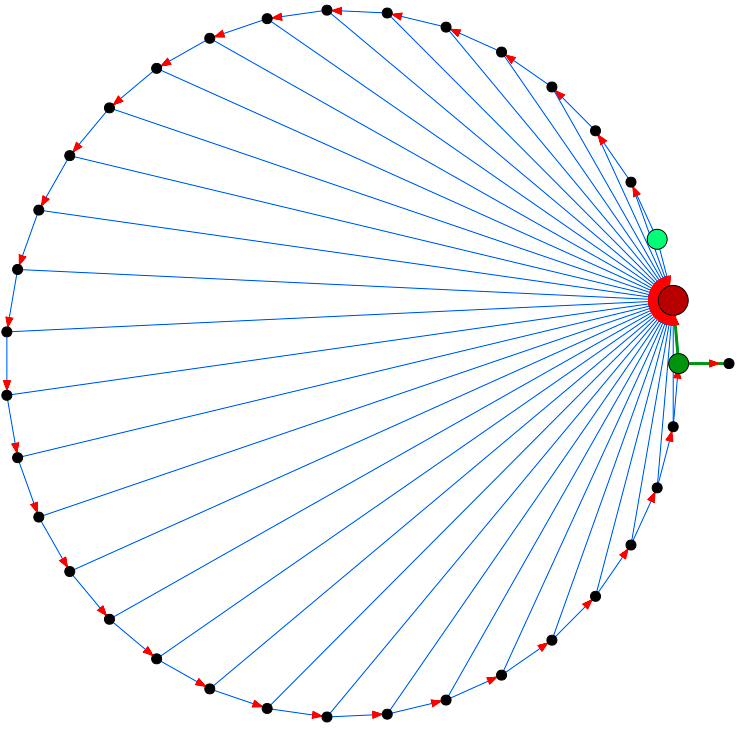
\includegraphics[height=2.2in]{../images/inf_reduction_graph_CIRCO.png}
	}
	\subfigure[Drawn using the Fdp algorithm.]{
		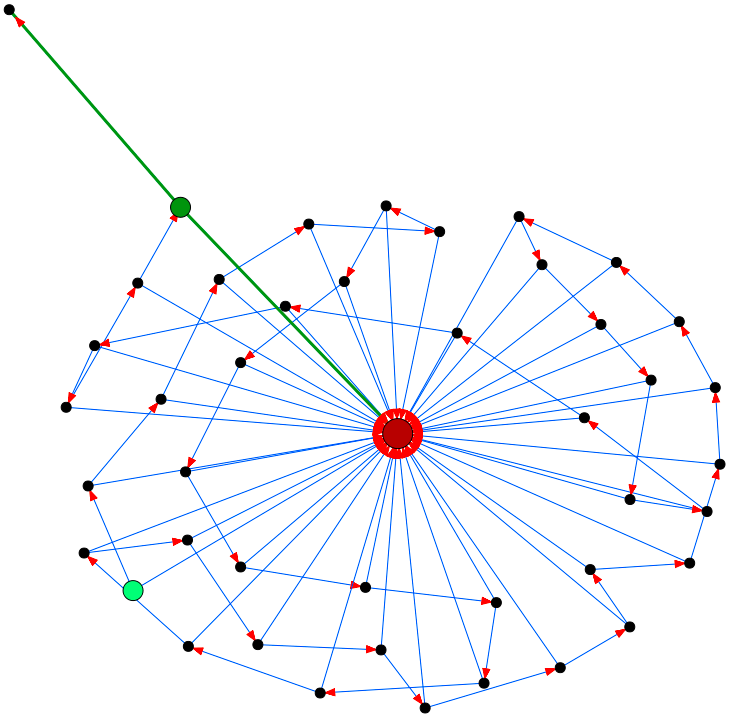
\includegraphics[height=2.2in]{../images/inf_reduction_graph_FDP.png}
	}
	\caption
	[$(\lam{a}{b}) (\lam{x}{(xxx)} \lam{y}{(yyy)})$]
	{$G_\beta\big((\lam{a}{b}) (\lam{x}{(xxx)} \lam{y}{(yyy)})\big)$. The normal form is drawn
	as a larger node. This is one generation of the reduction graph, but it 
	continues ad infinitum.}
	\label{fig:images_inf_reduction_graph}
\end{figure}


% Flere eksempler?

\section{Non-planarity}

As a consequence of Lemma \ref{lem:complete} we know that in the general case,
a reduction graph can contain as its subgraph $K_5$, whence the graph is
non-planar according to Kuratowski's theorem. Thus, it is in general not
possible to planarize a reduction graph. In Figure \ref{fig:images_lambda_k5}
a reduction graph whose underlying undirected graph \emph{is} $K_5$ is shown.

\begin{lemma}\label{lem:complete}
	$\forall n\in\N:\ \exists M\in\Lambda$ such that the $\beta$-reduction graph of $M$
	contains the complete (undirected) graph of $n$ nodes, $K_n$.
\end{lemma}
\begin{proof}[Proof (after a sketch by Jakob Grue Simonsen)]
	Let $n\in\N$, and let $M\in\Lambda$ be
	\begin{equation*}
		(\lam{x_1}{y}) ((\lam{x_2}{y}) ((\lam{x_3}{y})\hdots(\lam{x_{n}}{y})))
	\end{equation*}
	where $x_1\hdots x_n$ are distinct variable names. $M$ has $n-1$ distinct reducts of the form
	\begin{align*}
		&(\lam{x_1}{y}), \\
		&(\lam{x_1}{y})((\lam{x_2}{y}) y), \\
		&(\lam{x_1}{y})((\lam{x_2}{y}) ((\lam{x_3}{y}) y)),\ \hdots
	\end{align*}
	Call them $r_1,\hdots,r_{n-1}$ from least to greatest. For every
	$1\leq i < j \leq n-1$ we have $r_j\barrow r_i$. Thus, since $M\barrow r_i$ 
	for $1\leq i \leq n-1$, we have for every pair $(N_0,N_1)$ in the $\beta$-reduction 
	graph that $N_0\barrow N_1$ or $N_1\barrow N_0$, whence the underlying 
	undirected graph of the reduction graph is $K_n$.
\end{proof}

\begin{figure}[htpb]
	% (#x1.(y)) ((#x2.(y)) ((#x3.(y)) ((#x4.(y)) (#x5.(y)))))
	\centering
	\subfigure[Drawn using the Neato algorithm.]{
		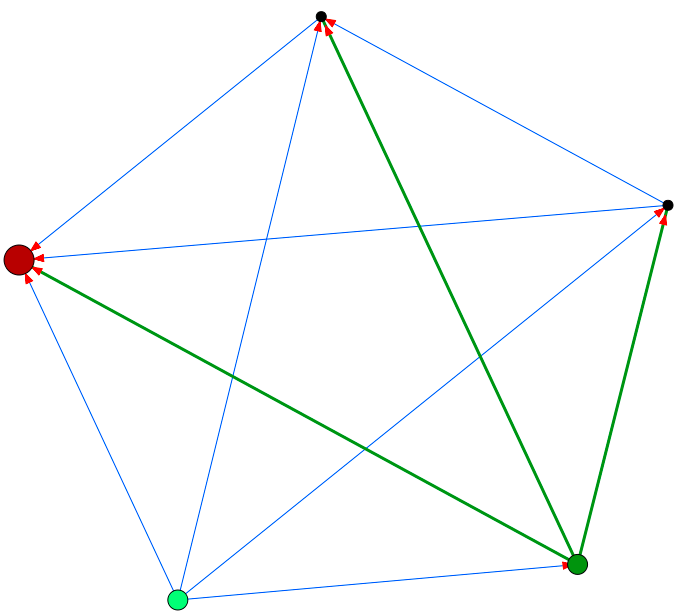
\includegraphics[height=2.2in]{../images/lambda_k5_NEATO.png}
	}
	\subfigure[Drawn using the Dot algorithm.]{
		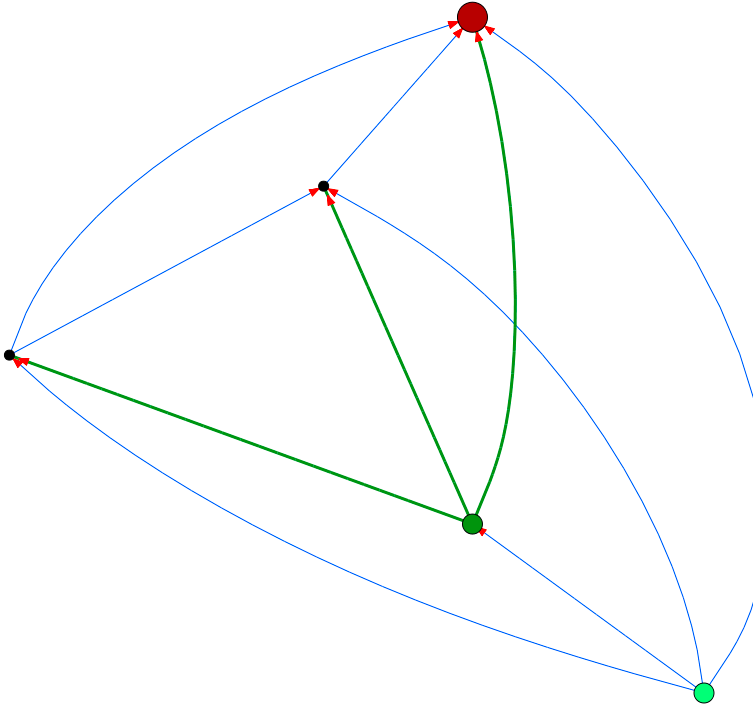
\includegraphics[height=2.2in]{../images/lambda_k5_DOT.png}
	}
	\caption
	[$(\lam{x_1}{y}) ((\lam{x_2}{y}) ((\lam{x_3}{y}) ((\lam{x_4}{y}) (\lam{x_5}{y})))$]
	{$G_\beta\big((\lam{x_1}{y}) ((\lam{x_2}{y}) ((\lam{x_3}{y}) ((\lam{x_4}{y}) (\lam{x_5}{y}))))\big)$
	from the proof of Lemma \ref{lem:complete}.}
	\label{fig:images_lambda_k5}
\end{figure}

\section{In- and out-degree of nodes}

The in- and out-degree of nodes varies a lot; the amount of redexes can be
very different from term to term, resulting in varying out-degrees, while some
nodes can have a potientially infinitely high in-degree.

For example, in the reduction graph for the term $(\lam{a}{b}) (\lam{x}{(xxx)}
\lam{y}{(yyy)})$, every node has an out-degree equal to 2 and an in-degree of
1, except the nodes representing the normal form and the initial term. The
former has an infinitely high in-degree and an out-degree of 0, the latter has
an in-degree of 0. The graph is illustrated on Figure \ref{fig:images_inf_reduction_graph}.

Since a particular lambda term in a reduction graph is finite, it necessarily has
a finite amount of redexes. The out-degree of the nodes representing the terms
is therefore finite.

% #a.(b) (#x.((x x) x) #y.((y y) y)) #a.(b) (#x.((x x) x) #y.((y y) y))
% #a.(b) ((#x.((x x) x) #y.((y y) y)) (#x.((x x) x) #y.((y y) y)))
% #a.(b) ((#a.(b) (#x.((x x) x) #y.((y y) y))) (#x.((x x) x) #y.((y y) y)))
% (#x1.(y)) ((#x2.(y)) ((#x3.(y)) ((#x4.(y)) (#x5.(y)))))

% Den her ser ret sej ud omkring nr. 100!
% #f.(#x.(f (x x))) (#x.(f (x x))) #y.((y y) y)

\fact Nodes can have an infinitely high in-degree.

\fact Nodes have a finite out-degree.

\fact The node representing the initial term can have an in-degree of 0.

\fact Since there always exists a path from the start node to all other nodes
in the reduction graph, the underlying undirected graph of a $\beta$-reduction
graph is connected. Hence, if there exists a node with an in-degree of 0, it
is the initial node.

\begin{figure}[tpb]
	% (#x.((x x) x) #y.((y y) y))
	\centering
	\subfigure[Drawn with the Neato algorithm.]{
		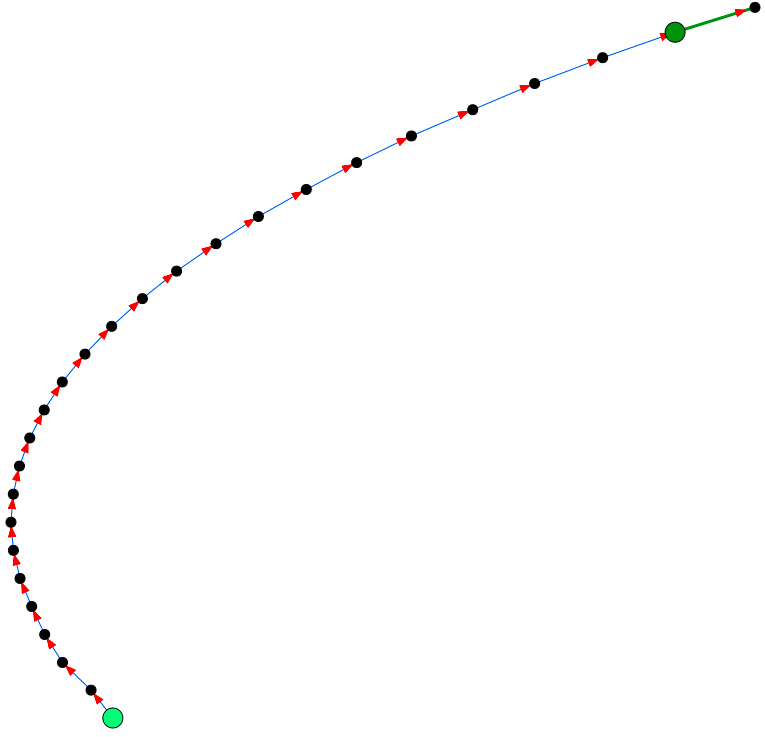
\includegraphics[height=2.2in]{../images/inf_reduction_graph_2_NEATO.png}
	}
	\subfigure[Drawn with the Fdp algorithm.]{
		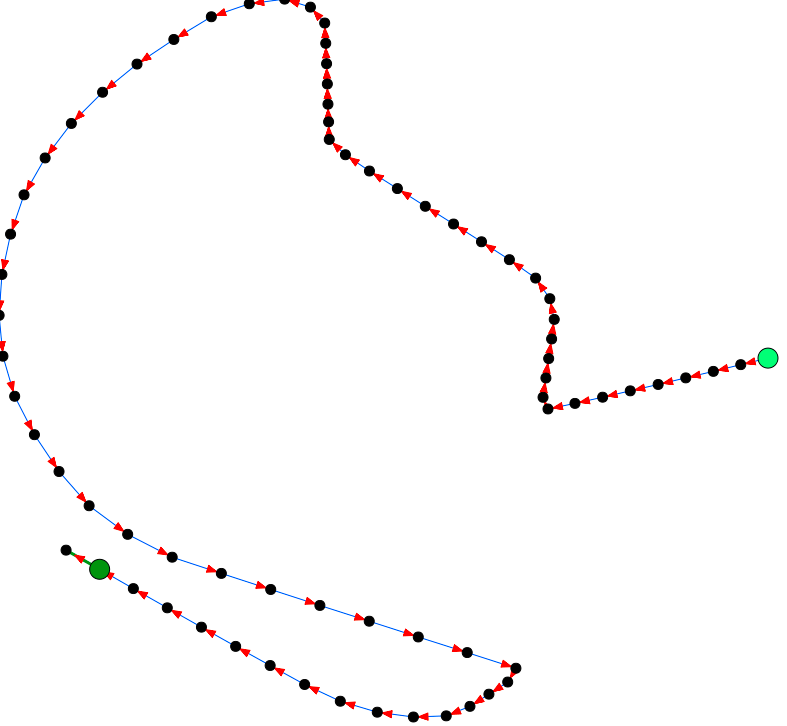
\includegraphics[height=2.2in]{../images/inf_reduction_graph_2_FDP.png}
	}
	\caption
	[$\lam{x}{(xxx)} \lam{y}{(yyy)}$]
	{$G_\beta\big(\lam{x}{(xxx)} \lam{y}{(yyy)}\big)$}
	\label{fig:images_inf_reduction_graph_2}
\end{figure}

\section{Normal Forms}

If the term whose reduction graph is visualized has a normal form, it is
desirable to be able to easily see it, even when there are a lot of nodes in
the graph. Therefore, a clear graphical hint must be added to the node that
represent a normal form. This could for instance be implemented as giving the
normal form node a certain colouring, a certain size or draw it with a
different shape than the other nodes (e.g. square vs. circular).

\fact Regardless of whether a term has a normal form or not, the amount
of edges and nodes in its reduction graph can be infinite; see for instance Figure 
\ref{fig:images_inf_reduction_graph_2} and \ref{fig:images_inf_reduction_graph}.
Similarly, both terms with and without normal forms can have finite reduction graphs;
see e.g. Figure \ref{fig:images_lambda_k5} and \ref{fig:images_Circle_1}.

% \fact Terms without normal forms have reduction graphs with infinitely many
% nodes and edges (e.g. the graph in Figure \ref{fig:images_inf_reduction_graph_2}). 
% 
% \fact Terms with normal forms have possibly infinite reduction graphs (e.g.
% the graph in Figure \ref{fig:images_inf_reduction_graph}).

%!TEX root = ../rapport.tex

\chapter{Look of the Graph Drawings}

In this Chapter we present the thoughts on the look of the generated drawings
and the decisions we made concerning colouring, sizing, etc.

\section{Direction}

The graphs are directed, so some kind of arrow heads need to be drawn. Since
an edge can be drawn spanning a lot of screen area, the type of arrow has to
be designed such that it is clear to see where an edge starts from the arrow
head alone and vice versa. An alternative to arrows is drawing the edges with
a colour gradient. In this approach, an edge would be couloured e.g. green at
the start and red at the end, interpolating the colours on the edge line. 

A study of the usability of these and other methods is presented in
\cite{Holten2009}. In this study, the representation that performed best was
the so-called ``tapered'' representation, ``[...] in which the width of an
edge is gradually varied along its length -- wide at the start and narrow at
the end [...]'' \cite[p. 2307]{Holten2009}. The authors recommend avoiding the
intuitive representation, where a ``normal'' arrowhead is drawn, altogether.
Nonetheless, for our purposes, we found that the regular arrow heads gave
reasonable results, and they have the benefit that they are easy to implement.
In a future version of the software alternatives to this approach could be
explored.

\section{Edge Weighting}

As seen in Chapter \ref{chap:theory} there can be more than one edge between
two nodes in a $\beta$-reduction graph. We have chosen not to display this
information and instead draw each connection between nodes for terms $M$ and
$N$ as a single line, regardless of whether there are one or several ways to
reach term $N$ from term $M$. This is done in an effort to reduce the visual
clutter in the drawing; for terms with e.g. 10 redexes that all have the same
constractum it would be distracting to see 10 lines on the drawing, all of
them between the same two nodes. For instance, the term $M_{K_{10}}$ below has
several redexes that all have the same contractum, $y$:
\begin{equation*}
	M_{K_{10}} \equiv
	(\lam{x_1}{y}) 
	((\lam{x_2}{y}) 
	((\lam{x_3}{y}) 
	((\lam{x_4}{y}) 
	((\lam{x_5}{y}) 
	((\lam{x_6}{y})
	((\lam{x_7}{y})
	((\lam{x_8}{y})
	((\lam{x_9}{y})
	(\lam{x_{10}}{y}))))))))) \barrow y
\end{equation*}
An alternative would be to annotate each line with its ``weight'', i.e. write
``10'' on the line. However, in a drawing of a reduction graph with e.g. 50
edges lying in close proximity to each other, these numbers could easily get
mixed up.
\begin{figure}[htbp]
	% (#x1.(y)) ((#x2.(y)) ((#x3.(y)) ((#x4.(y)) ((#x5.(y)) ((#x6.(y)) ((#x7.(y)) ((#x8.(y)) ((#x9.(y)) ((#x10.(y)))))))))))
	\centering
		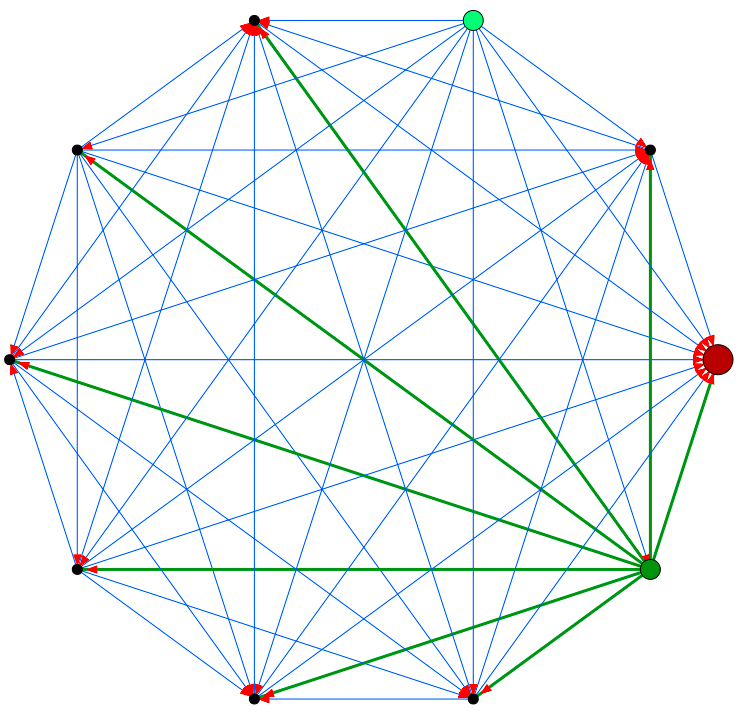
\includegraphics[height=2in]{../images/lambda_k10_CIRCO.png}
	\caption
	[$M_{K_{10}}$, a reduction graph version of $K_{10}$.]
	{$G_\beta(M_{K_{10}})$, drawn with the Circo algorithm.}
	\label{fig:images_lambda_k10_CIRCO}
\end{figure}

\section{Colouring}

To be able to distinguish between different kinds of nodes in the reduction graph,
different variants of colouring and sizing are used:
\begin{itemize}
	\item The normal form, if any, must be easily recognizable. Therefore it is
	coloured red and drawn as the biggest node: 
\includegraphics[height=0.2in]{../images/NF_example.png}.
	
	\item The start term is represented by a light green, medium sized node: 
	
\includegraphics[height=0.12in]{../images/STARTNODE_example.png}.
	This makes it easy to recognize
	
	\item The current term that is being ``expanded'', that is, having all its
	redexes reduced to their contracta, is coloured dark green and made medium size:
	
\includegraphics[height=0.12in]{../images/CURRENTNODE_example.png}.
	Also, all the edges representing reductions are drawn thicker than the other edges
	and in the same dark green colour as the node.
	
	\item Regular nodes in the reduction graph are drawn as small, black dots.
	Edges representing reduction that are not the ``current'' reduction are
	drawn as thin, blue lines.
	
	\item All self-referencing nodes, i.e. nodes with an edge that is both outgoing 
	and ingoing, are drawn as red squares: 
\includegraphics[height=0.1in]{../images/redsquare_example.png} . 
	If the start term is self-referencing,
	it is drawn as a light green, medium sized circle with a red square inside.
	
	\item The arrow heads on the edges are bright red, making them easily 
	distinguishable in a cluttered drawing.
	
	\item To make it easier to quickly see where the contracta of a given node are,
	all its outgoing edges are highlighted by being drawn with thicker lines
	when it is clicked, see Figure \ref{fig:images_highlighted_node_DOT}. 
	This only happens if the node has been expanded. Only one node can have 
	its edges highlighted at a time, so all previously highlighted edges are 
	reverted to their normal look if a new node is clicked. 
\end{itemize}
\begin{figure}[htbp]
	% #B1.((((#B2.(#B3.(#B4.(B2))) (#B5.(#B6.(#B7.(#B8.(B1)))) #B9.((#B10.((#B11.(B9) #B12.(#B13.(#B14.(#B15.(B1)))))) #B16.(F1))))) #B17.(B1)) #B18.((#B19.(#B20.(B19)) (#B21.(B21) ((B1 #B22.(#B23.(B22))) #B24.(#B25.(#B26.((#B27.(B25) B25))))))))))
	\centering
	\subfigure[Drawn with the Dot algorithm.]{
		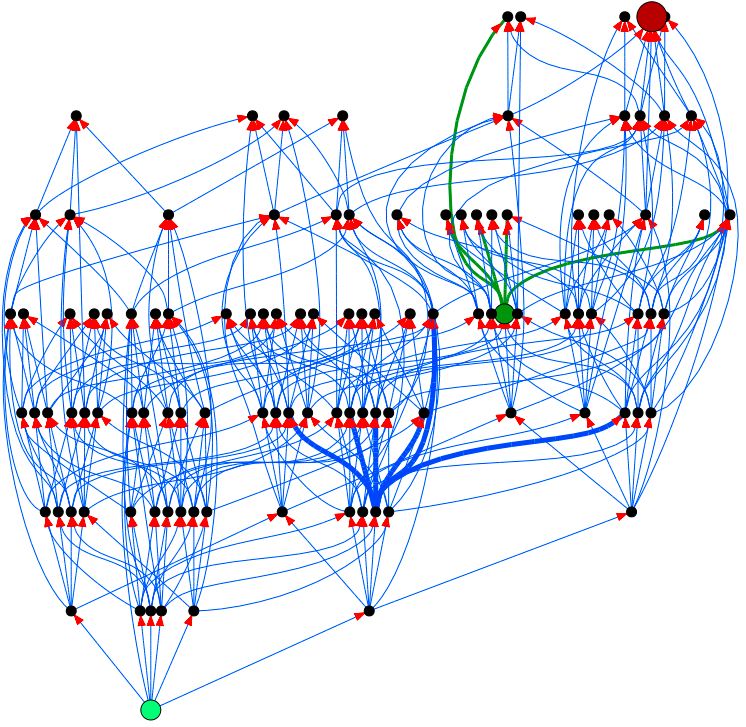
\includegraphics[height=2.5in]{../images/highlighted_node_DOT.png}
	}
	\subfigure[Drawn with the Neato algorithm.]{
		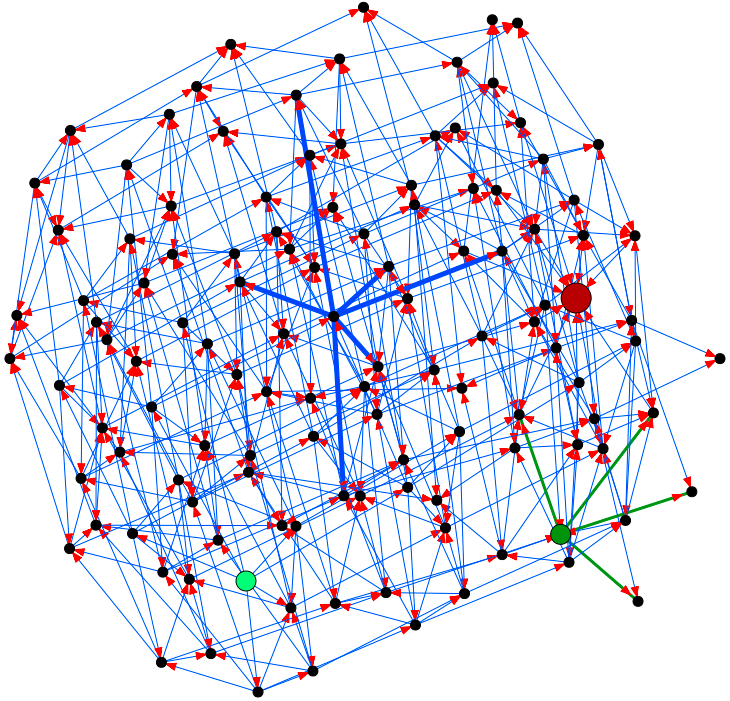
\includegraphics[height=2.5in]{../images/highlighted_node_NEATO.png}
	}
	\caption
	[Complex, 27-abstractor lambda term.]
	{A complex lambda term with 27 abstractors with a node and its outgoing
	edges highlighted.}
	\label{fig:images_highlighted_node_DOT}
\end{figure}

%!TEX root = ../rapport.tex

\chapter{Implementation}
\label{chap:implementation}

In this Chapter we will briefly discuss the implementation of the concepts
presented in the preceding Chapters. The presentation here is only
superficial; for details the actual source code should be consulted.

\section{Representation of Lambda Terms}

A lambda term is represented as a directed acyclic graph (DAG). The nodes of the
DAG are encoded in Python as objects. There are three types of nodes: 
abstraction, application and variable:
\begin{description}
	\item[Abstraction nodes] define scopes for bound variables and can be thought
	of as the encoding of the $\lambda$s in the DAG-structure. This node type
	always has one child.
	
	\item[Application nodes] have two children. The first of these
	is either the DAG-representation of some \emph{active} subterm of 
	$M$, or another application node. The second child is the DAG-representation
	of the ``argument'', that is, the lambda term that are to be substituted
	in place for a bound variable. An application node represents a possible
	one-step $\beta$-reduction.
	
	\item[Variable nodes] represent free or bound variables. A bound 
	variable is associated with a scope, represented by an ancestral
	abstraction node. Variable nodes cannot have descendants.
\end{description}

This representation is straightforwardly encoded in Python with a general node
class, \pycode{LambdaNode}, which has a subclass for each node type.
\begin{itemize}
	\item Each \pycode{LambdaNode}-object maintains pointers to its immediate 
	descendants as well as a pointer to its parent node.
	
	\item The abstraction nodes furthermore maintain a list of pointers to the
	variable nodes that represent the variables bound by this particular abstractor.
	These variable nodes must be descendants of the abstraction node, although 
	not necessarily direct descendants.
	
	\item Every abstraction node knows the name of the variable that it binds.
	This is done in order to be able to easily build the list of bound 
	variables after parsing a string representation of a lambda term. When
	the list of variables has been built, this name is not important anymore, 
	but it still serves as a means of producing human-readable output of the DAG.
	
	\item When a term is reduced, the problem is attacked ``top-down'', i.e. we first
	see the abstraction node, and then we have to deal with its variables.
	Therefore there is no need for a doubly linked connection between abstraction
	nodes and variable nodes, and we can safely encode the relationship as a simple
	list of bound nodes in each abstraction node.
	
	\item The comparison of lambda terms have to follow Convention \ref{con:alpha} regarding
	$\alpha$-congruence. Two DAGs are compared by their \emph{normalized} string representations,
	which simply is the lambda term with all
	variables renamed in a systematic, well-defined way, such that if two terms
	are equal modulo $\alpha$-congruence, then their normalized string representations will
	be the same.
\end{itemize}

A term that is not in $\beta$-normal-form has at least one $\beta$-contractum,
and therefore the DAG-re\-pre\-sen\-ta\-tion of that term contains at least one
application node and one abstraction node. More specifically, for each
possible one-step $\beta$-reduction in a term $M$, its DAG will contain one
application node. The first descendant of this node will be an abstraction
node, while the second, ``rightmost'', descendant will be the argument that
will be applied to the function represented by the abstraction node.

\section{Parsing}

We have implemented a parser that generates the aforementioned representation
for the grammar specified in Definition \ref{def:grammar} with a few subtle
differences. First of all, the symbol used for $\lambda$ is a \texttt{\#}.
Secondly, all lambda expressions fed into the parser are run through a
preprocessing step that adds all implied parentheses to the string. This step
is included to make the parser definition itself simpler. The preprocessing
step ensures that Conventions \ref{con:assoc} and \ref{con:extent} are
followed.

We used a parser generator to make the parser, since we found it simpler and
more straightforward than to implement it from scratch. There exist numerous
parser generators for Python \cite{pythonParserGeneratorList}. We chose YAPPS2
(Yet Another Python Parser System 2) \cite{YAPPS2} because it is designed such
that it generates human-readable code. YAPPS2 takes a specification of an
LL(1) grammar and writes the Python code for the corresponding parser.

\section{Representation of $\beta$-reduction Graphs}

A reduction graph is represented in Python as an instance of the
\pycode{Graph}-class. A \pycode{Graph}-object contains its nodes, represented
as instances of the \pycode{Node}-class, in three different data structures:
\begin{enumerate}
	\item A dictionary with references to the nodes, where the keys are normalized string 
	representations of the lambda terms represented by the nodes.
	
	\item Another dictionary with references to the same nodes, but keyed on the
	names of the nodes instead of the lambda terms.
	
	\item A list of the nodes. This is included to ensure that the nodes can be
	accessed in a consistent ordering, since the Python function \pycode{dict.items()}
	returns the elements of the dictionary in an arbitrary order.
\end{enumerate}
A \pycode{Graph}-object contains exactly one \pycode{Node} for each lambda
term in the reduction graph; if one tries to add a node for an existing term,
nothing happens.

A \pycode{Node}-object has a name and a reference to the lambda term which it
represents. It furthermore has a list of its children and a list of its
parents. These lists contain instances of the \pycode{Edge}-class, which
basically just implements a coupling between two \pycode{Node}-objects.

\section{Generation of $\beta$-reduction Graphs}

In the file \texttt{operations.py}, the functions necessary for the generation
of reduction graphs are implemented. The main function here is
\pycode{reductiongraphiter()} which returns an iterator over the different
``generations'' of the reduction graph. Each generation is a reduction graph
containing everything from the generation immediately before, along with the
contracta of all the redexes of one term that was not reduced in the graph of
the preceding generation. Thus, the longer one iterates, the bigger and more
complete a reduction graph is returned. 

The function takes three arguments: the lambda term in whose reduction graph
we are interested, a start parameter controlling when the iterator should
start emitting graphs (making it possible to return e.g. only the ten last
generations) and an end parameter that controls how long the computation shall
continue, i.e. how many terms should be reduced. Note that, in general, a
``large'' end value is preferred, since it allows the user to continue to step
forwards. Therefore, the value used in practice in the implementation is fixed
to $10^6$.

{\textcolor{black}
In the case of reduction graphs of infinite size, the computation only halts
when the given maximum is reached. For finite graphs, the computation halts
either when the maximum is reached or when the graph is fully computed,
depending on the chosen maximum value.

Each time a reduction graph is returned by Pythons \pycode{yield}-statement, a
deep copy operation is performed. This is done in order to ensure that later
stages in the program indeed see the different generations of graphs as
distinct objects, instead of a collection of references to the same set of
\pycode{Node}s. The built-in copy operation \pycode{copy.deepcopy()} proved to
be too slow, therefore a custom deep copy operation was implemented.
}
\section{Drawing Algorithms}

All drawing algorithms are implemented as classes extending the
interface-style class \pycode{DrawingAlgorithm}. The drawing functions use
only those methods that are defined in \pycode{DrawingAlgorithm}, so to extend
the software with new algorithms, the only necessity imposed is that this
interface is implemented. For instance, the algorithms that we provide are
implemented in two ways: algorithms using the software package GraphViz
\cite{GraphViz} and a ``home-cooked'' implementation. The actual code provided
by us for the GraphViz-algorithms are merely a layer that calls the underlying
GraphViz-routines and ensures compatibility with the graph representations
that we use.

GraphViz is a tool meant for ``end-to-end'' treatment of graph drawing, i.e.
it has a graph description language and features for different graphic output
modes with different shapes for nodes etc. The only property relevant for us
is the node positions, so when running the algorithms from GraphViz we first
convert our graph model into GraphViz's format, ask GraphViz to compute the
node positions and finally copy them into our model. 

A common task when working with graphs and drawing algorithms is to find the
graph-theoretical distance between all pairs of nodes. It is used in the
algorithm that we implemented ourselves, and it is highly likely that a new
algorithm needs this functionality too. An implementation of the all-pairs
distance algorithm from \cite{Seidel1992} is available for future use.

The following drawing algorithms are implemented:
\begin{description}
	\item[Majorization] is an implementation of the algorithm by Gansner et al. 
	described in \cite{Gansner2004} that makes heavy use of the NumPy library \cite{NumPy}. 
	It is a force-based approach that uses stress majorization
	to minimize an energy function. This algorithm is also implemented in the GraphViz
	package, but there are several reasons to why we chose to make our own implementation:
	\begin{itemize}
		\item we have complete control with the algorithm, allowing us to tweak it;
		\item for the same reason we are able to call functions to update the screen
		when we see fit, allowing us to create an animation-like look.
	\end{itemize}
	
	This is the only non-GraphViz algorithm implemented.
	
	In the program it is called ``Neato Animated''.

	\item[Neato] is GraphViz's implementation of the algorithm by Gansner et al. 
	Since it behaves like a ``black box'', it uses its own settings for the
	stress function which we cannot change. This function has been modified in our
	own implementation.
		
	\item[Dot] is an algorithm that makes a hierachichal layout of a graph. As the only
	algorithm implemented, it does not necessarily draw straight lines for edges; it computes
	a (possibly straight) B\'ezier curve for the edges. Like the other algorithms except ``Majorization''
	it is really a layer on top of the GraphViz-module Dot.
	
	\item[Circo] performs a circular layout of the nodes. It is an implementation of 
	the algorithm described in \cite{Six1999}.
	
	\item[Twopi] also performs a circular layout, but it places the nodes on several circles instead
	of only one as Circo does. 
	
	\item[Fdp] is another force-based algorithm. It is an implementation of 
	the algorithm described by Fruchterman et al. \cite{Fruchterman1991}.
\end{description}

\section{Graphical User Interface}

The focus of this work has not been on the design of a graphical user
interface. However, in order to make the program accessible, a draft user
interface has been implemented. We have chosen to use the widget library GTK
\cite{PyGTK}, since it runs on several platforms and is already widely used in
e.g. the Gnome desktop environment.

Sometimes the layout algorithms place the nodes in a suboptimal way compared
to the users perception of the graph. Because of this, it is possible to drag
and manually reorder the nodes in the graph. Some algorithms tries to optimize
the graph layout after the node has been dragged, while others simply let the
user move the nodes around. This difference exists because the algorithms are
very different in nature, and on some of the algorithms an optimization of a
reordered graph would completely render the manual reordering obsolete.
%!TEX root = ../rapport.tex

\chapter{Results}
\newcommand{\exampleheight}{2.2in}

The program implemented is able to draw illustrations of reduction graphs with
several different drawing algorithms. This Chapter contains examples of reduction graphs
drawn by the software. 

The graphs were produced ``randomly'', by experimenting with lambda terms and
adjusting them to exhibit (sometimes) interesting behaviour in their reduction
graphs. We found that the best all-round drawing algorithm to use when
experimenting with terms is the Neato algorithm, since it gives nice graphs
most of the time; the others can give very beautiful graphs sometimes, but
often their output is worse than that of Neato.

For each example graph, the caption text contains an explanation of what is
going on. Thus, the contents of this Chapter is solely to be found in the
images and their captions.

\begin{figure}[htbp]
	% #a.(b) (#x.((x x) x) #y.((y y) y))
	\centering
	\subfigure[Drawn with Dot.]{
		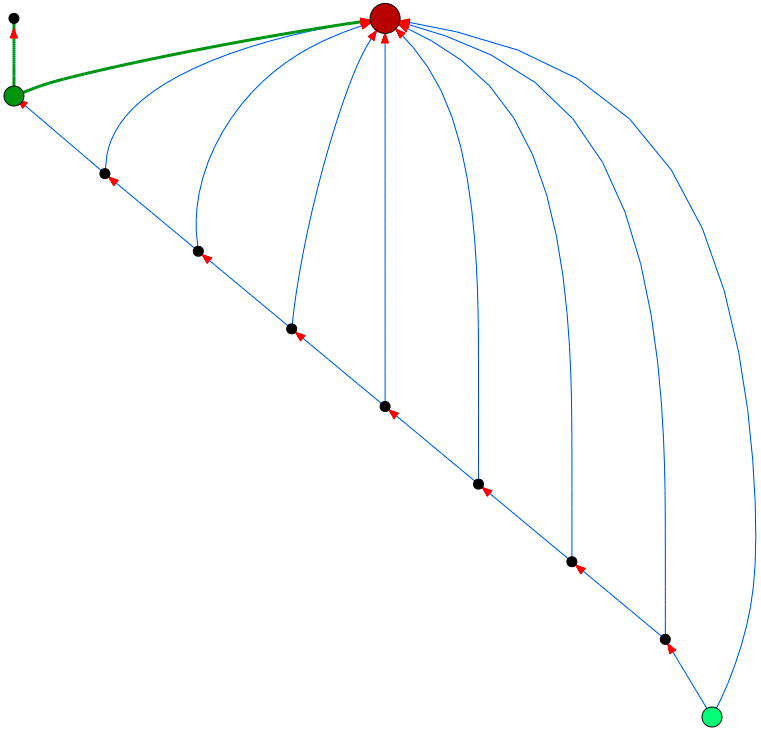
\includegraphics[height=\exampleheight]{../images/inf_reduction_graph_DOT.png}
	}
	\subfigure[Also drawn with Dot, but several generations later.]{
		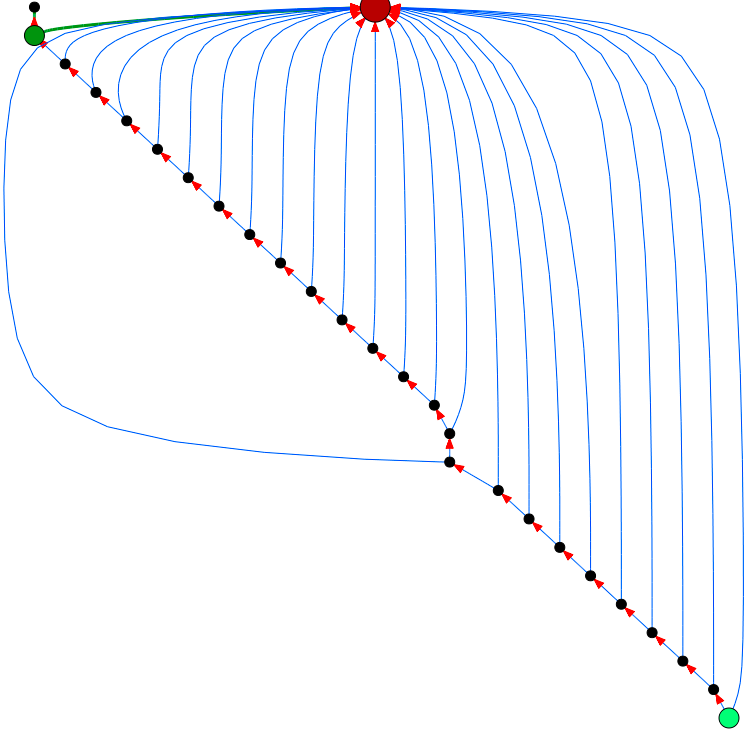
\includegraphics[height=\exampleheight]{../images/inf_reduction_graph_DOT2.png}
	}
	\caption[$(\lam{a}{b}) (\lam{x}{(xxx)} \lam{y}{(yyy)})$]
	{When Dot draws the graph $G_\beta\big((\lam{a}{b}) (\lam{x}{(xxx)} \lam{y}{(yyy)})\big)$
	for later generations, a peculiar phenomenon occurs: one of the nodes on the ``ladder''
	has one of its edges pointing in another way than the equivalent edges of the other
	nodes. This is an artefact of the internal workings of the Dot algorithm.}
	\label{fig:images_inf_reduction_graph_DOT}
\end{figure}

\begin{figure}[htbp]
	% #f.(#x.(f (x x))) (#x.(f (x x))) #y.((y y) y)
	\centering
	\subfigure[Neato.]{
		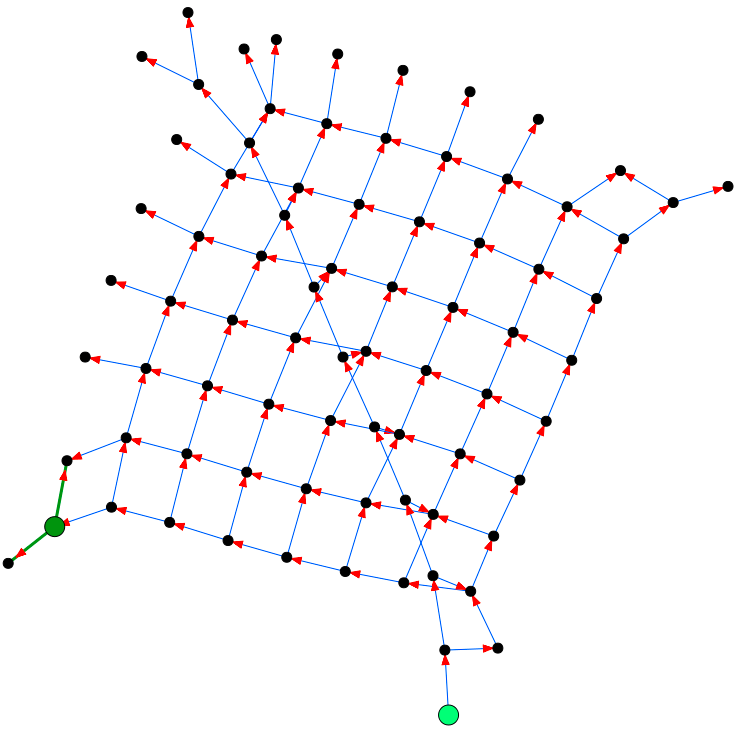
\includegraphics[height=\exampleheight]{../images/Ycomb_1_NEATO.png}
	}
	\subfigure[Twopi.]{
		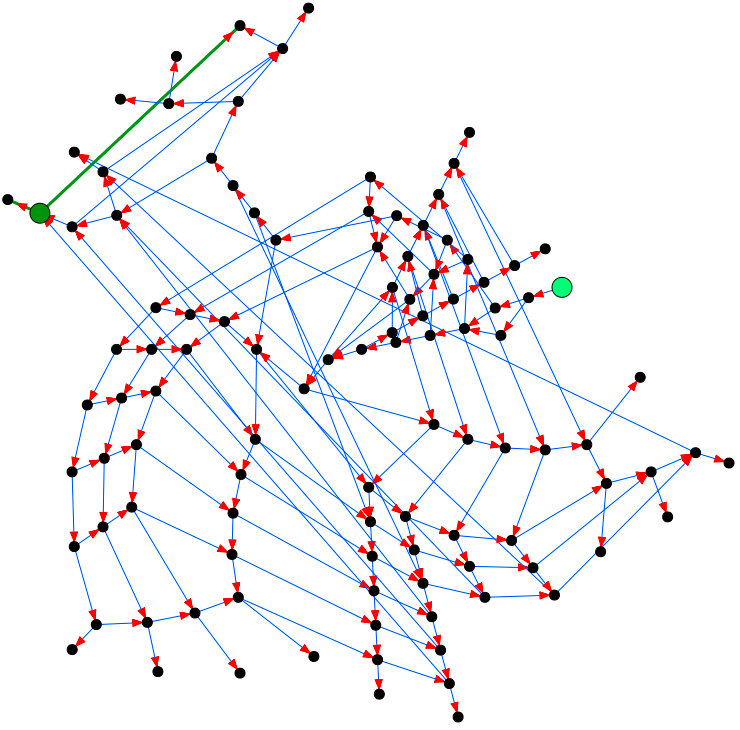
\includegraphics[height=\exampleheight]{../images/Ycomb_1_TWOPI.png}
	}
	\subfigure[Dot.]{
		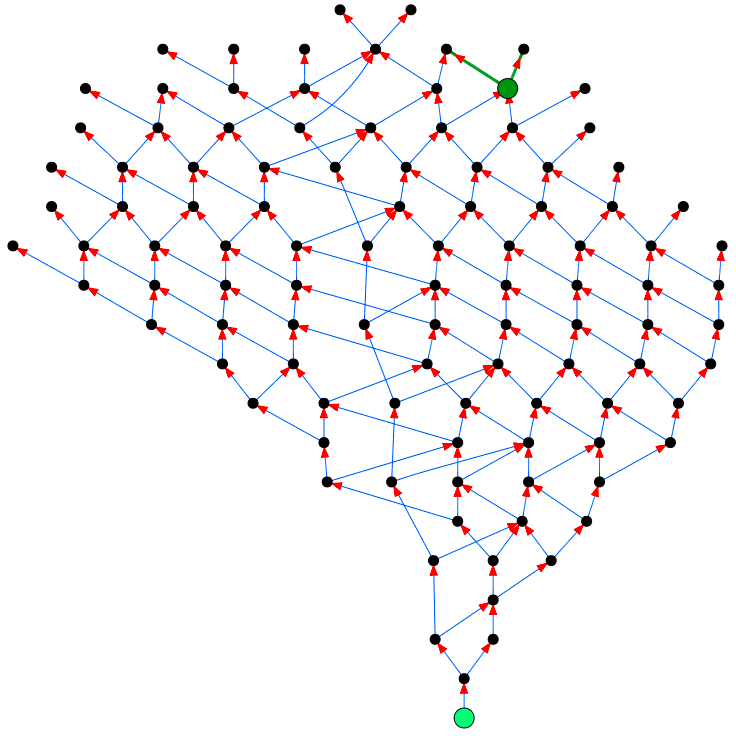
\includegraphics[height=\exampleheight]{../images/Ycomb_1_DOT.png}
	}
	\caption[$(\lam{f}{(\lam{x}{f (x x)}) (\lam{x}{f (x x)})}) \lam{y}{(y y) y}$]
	{The Y-combinator applied to $\omega_3$: $G_\beta\big((\lam{f}{(\lam{x}{f (x x)}) (\lam{x}{f (x x)})}) \lam{y}{(y y) y}\big)$.}
	\label{fig:images_YComb_1}
\end{figure}

\begin{figure}[htbp]
	% ((#b1.(b1) #b2.((#b3.(b2) #b4.((#b5.(b2) b4))))) #b6.((#b7.(b6) #b8.(#b9.(#b10.(#b11.(b11)))))))
	\centering
	\subfigure[Neato]{
		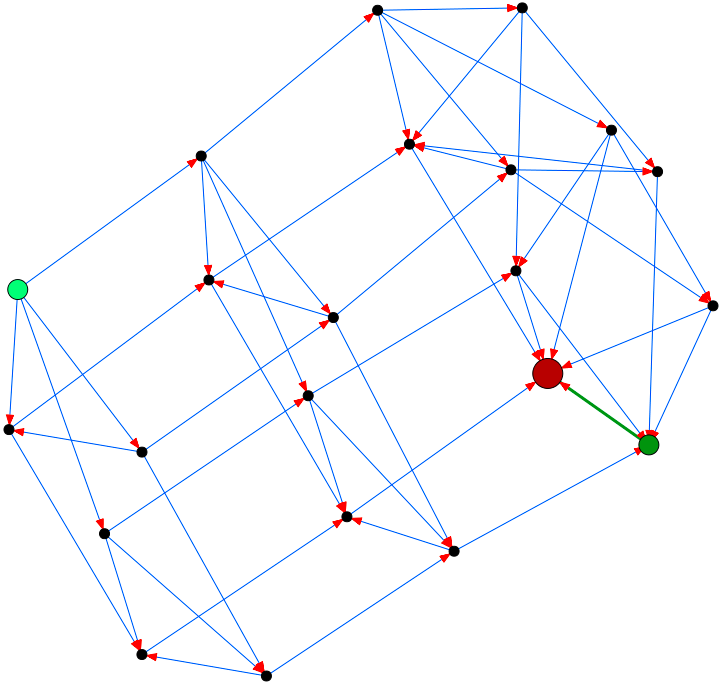
\includegraphics[height=\exampleheight]{../images/finite_ex_1_NEATO.png}
	}
	\subfigure[Dot]{
		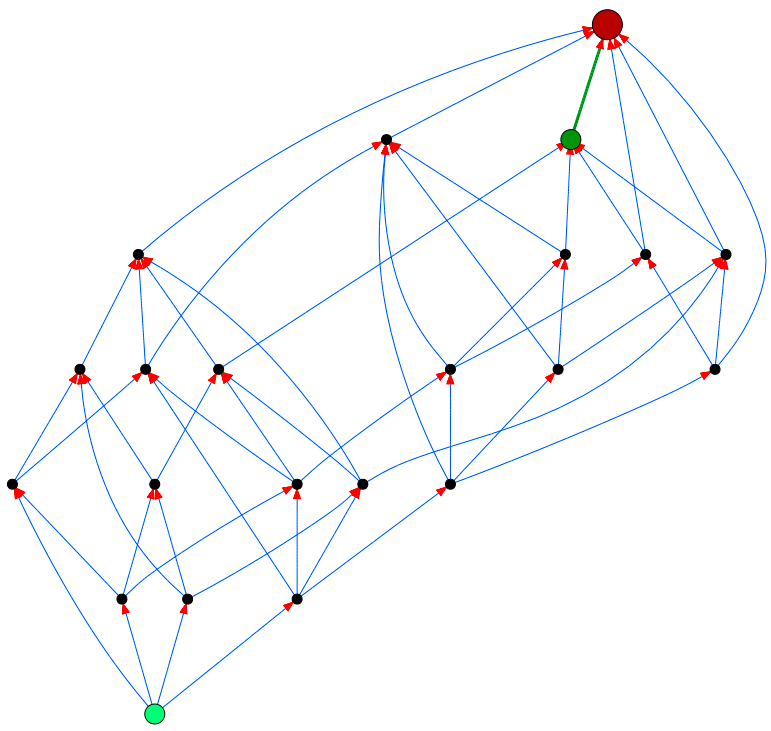
\includegraphics[height=\exampleheight]{../images/finite_ex_1_DOT.png}
	}
	\subfigure[Fdp]{
		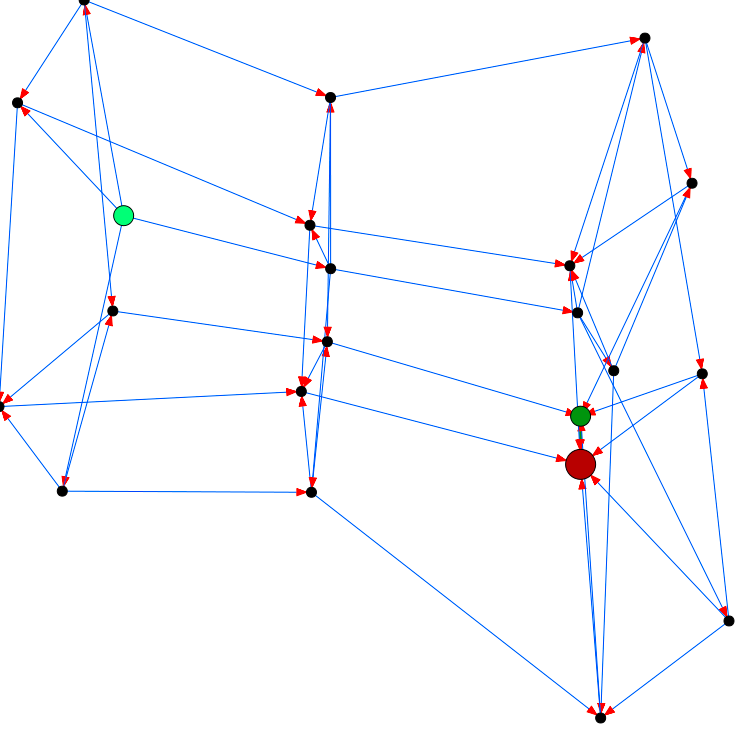
\includegraphics[height=\exampleheight]{../images/finite_ex_1_FDP.png}
	}

	\caption[$((\lam{x}{x}) \lam{y}{((\lam{z}{y}) \lam{z}{((\lam{a}{y}) z)})}) \lam{x}{((\lam{y}{x}) \lam{y}{(\lam{z}{(\lam{a}{\lam{b}{b}})})})}$]
	{This randomly generated lambda term has a box-like embedding of 
	its reduction graph: $G_\beta\big(((\lam{x}{x}) \lam{y}{((\lam{z}{y}) \lam{z}{((\lam{a}{y}) z)})}) \lam{x}{((\lam{y}{x}) \lam{y}{(\lam{z}{(\lam{a}{\lam{b}{b}})})})}\big)$.
	}
	\label{fig:images_finite_ex_1_NEATO}
\end{figure}

\begin{figure}[htbp]
	% (#B1.(#B2.(((#B3.(#B4.(#B5.(#B6.(B1)))) #B7.(#B8.(B7))) (#B9.(B1) #B10.(#B11.(B1)))))) (#B12.(#B13.(B13)) #B14.(#B15.(#B16.((#B17.(B17) B16))))))
	\renewcommand{\exampleheight}{2.5in}
	\centering
	\subfigure[Twopi]{
		\includegraphics[height=\exampleheight]{../images/finite_ex_2_TWOPI.png}
	}
	\subfigure[Circo]{
		\includegraphics[height=\exampleheight]{../images/finite_ex_2_CIRCO.png}
	}
	\subfigure[Dot]{
		\includegraphics[height=\exampleheight]{../images/finite_ex_2_DOT.png}
	}
	\subfigure[Fdp]{
		\includegraphics[height=\exampleheight]{../images/finite_ex_2_FDP.png}
	}
	\subfigure[Neato]{
		\includegraphics[height=\exampleheight]{../images/finite_ex_2_NEATO.png}
	}
	\subfigure[Majorization]{
		\includegraphics[height=\exampleheight]{../images/finite_ex_2_MAJOR.png}
	}
	
	\caption
	[$\lambda x.(\lambda y.((\lambda z.(\lambda a.(\lambda b.(\lambda c.x))) \lambda z.(\lambda a.z)) (\lambda y.x \lambda z.(\lambda a.x))
	)) (\lambda x.(\lambda y.y) \lambda x.(\lambda y.(\lambda z.(\lambda a.(a) z))))$]
	{Another randomly generated lambda term. In its reduction graph we
	get a clear impression of the differences between the provided drawing algorithms.
	$G_\beta\big(
	\lambda x.(\lambda y.((\lambda z.(\lambda a.(\lambda b.(\lambda c.x))) \lambda z.(\lambda a.z)) (\lambda y.x \lambda z.(\lambda a.x))
	)) (\lambda x.(\lambda y.y) \lambda x.(\lambda y.(\lambda z.(\lambda a.(a) z))))
	\big)$.}
	\label{fig:images_finite_ex_2_CIRCO}
\end{figure}

\begin{figure}[htbp]
	% λB1.((λB2.(λB3.((λB4.((B4 (λB5.(B1) λB6.(λB7.(B7))))) λB8.(B8)))) B1))
	\centering
	\subfigure[Majorization]{
		\includegraphics[height=\exampleheight]{../images/finite_ex_3_MAJOR.png}
	}
	\subfigure[Neato]{
		\includegraphics[height=\exampleheight]{../images/finite_ex_3_NEATO.png}
	}
	
	\caption
	[$\lambda x.(\lambda y.(\lambda z.(\lambda a.(a ((\lambda b.x) (\lambda c.\lambda d.d))) \lambda e.e)) x)$]
	{The two force-directed algorithms, Neato and Majorization, differ
	only on subtleties. $G_\beta\big(\lambda x.(\lambda y.(\lambda z.(\lambda a.(a ((\lambda b.x) (\lambda c.\lambda d.d))) \lambda e.e)) x)\big)$.}
	\label{fig:images_finite_ex_3_MAJOR}
\end{figure}

\begin{figure}[htbp]
	% #f.(#x.(f (x x))) (#x.(f (x x))) #y.(y y)
	\centering
	\subfigure[Circo]{
		\includegraphics[height=\exampleheight]{../images/Ycomb_2_CIRCO.png}
	}
	\subfigure[Majorization]{
		\includegraphics[height=\exampleheight]{../images/Ycomb_2_MAJOR.png}
	}
	
	\caption
	[$\lambda f.(\lambda x.(f (x x))) (\lambda x.(f (x x))) \lambda y.(y y)$]
	{The Y-combinator applied to $\omega$: $\lambda f.(\lambda x.(f (x x))) (\lambda x.(f (x x))) \lambda y.(y y)$.
	No normal form exists, but there is a node from which the reduction operation
	cannot ``escape'' when it is first met.}
	\label{fig:images_Ycomb_2_CIRCO}
\end{figure}
\begin{figure}[htbp]
	% #f.(#x.(f (x x))) (#x.(f (x x))) #x.#y.(y y x)
	\centering
	\subfigure[Majorization]{
		\includegraphics[height=\exampleheight]{../images/Ycomb_3_MAJOR.png}
	}
	\subfigure[Majorization, after more generations.]{
		\includegraphics[height=\exampleheight]{../images/Ycomb_3_MAJOR2.png}
	}
	\subfigure[Neato]{
		\includegraphics[height=\exampleheight]{../images/Ycomb_3_NEATO.png}
	}
	\subfigure[Neato, after more generations.]{
		\includegraphics[height=\exampleheight]{../images/Ycomb_3_NEATO2.png}
	}
	\subfigure[Circo]{
		\includegraphics[height=\exampleheight]{../images/Ycomb_3_CIRCO.png}
	}
	\subfigure[Circo one step further; the lone outlier node emits new pairs of nodes.]{
		\includegraphics[height=\exampleheight]{../images/Ycomb_3_CIRCO2.png}
	}
	
	\caption
	[$\lambda f.\lambda x.(f (x x)) (\lambda x.f (x x)) \lambda x.\lambda y.(y y x)$]
	{The Y-combinator applied to $\lambda x.\lambda y.(y y x)$: $\lambda f.\lambda x.(f (x x)) (\lambda x.f (x x)) \lambda x.\lambda y.(y y x)$.
	This graph has an interesting property in that it appears to have two ``modes'';
	one where the ``path'' is thick, or broad, and one where we see a simple line
	of nodes next to each other. In some of the graph embeddings the first part
	looks almost like a helix.}
	\label{fig:images_Ycomb_3_1}
\end{figure}

\begin{figure}[htbp]
	% #f.(#x.(f (x x))) (#x.(f (x x))) #x.#y.(y y x)
	\centering
	\subfigure[Dot]{
		\includegraphics[height=\exampleheight]{../images/Ycomb_3_DOT.png}
	}
	\subfigure[Dot, after more generations.]{
		\includegraphics[height=\exampleheight]{../images/Ycomb_3_DOT2.png}
	}
	\subfigure[Fdp]{
		\includegraphics[height=\exampleheight]{../images/Ycomb_3_FDP.png}
	}
	\subfigure[Fdp, after more generations.]{
		\includegraphics[height=\exampleheight]{../images/Ycomb_3_FDP2.png}
	}
	\subfigure[Twopi]{
		\includegraphics[height=\exampleheight]{../images/Ycomb_3_TWOPI.png}
	}
	\subfigure[Twopi, after more generations.]{
		\includegraphics[height=\exampleheight]{../images/Ycomb_3_TWOPI2.png}
	}
	\caption
	[$\lambda f.\lambda x.(f (x x)) (\lambda x.f (x x)) \lambda x.\lambda y.(y y x)$]
	{The same lambda term as in Figure \ref{fig:images_Ycomb_3_1}.}
	\label{fig:images_Ycomb_3_2}
\end{figure}


\begin{figure}[htbp]
	% #x.(#y.(#x.(#y.(#s.(s x y))) #x.(#y.y) (#x.(#y.(#s.(s x y))) x y))) #f.(#x.(f (f x))) #f.(#x.(f (f (f x))))
	% cons(2,3)
	\centering
	\subfigure[$cons(2,3)$: ]{
		\includegraphics[height=\exampleheight]{../images/Cons23_NEATO.png}
	}
	\subfigure[$cons(5,0)$: ]{
		\includegraphics[height=\exampleheight]{../images/Cons50_NEATO.png}
	}
	\subfigure[$cons(4,4)$: ]{
		\includegraphics[height=\exampleheight]{../images/Cons44_NEATO.png}
	}
	\begin{tabular}{ll}
		$cons(2,3)$	& $\lambda x.(\lambda y.(\lambda x.(\lambda y.(\lambda s.(s x y))) \lambda x.(\lambda y.y) (\lambda x.(\lambda y.(\lambda s.(s x y))) x y))) \lambda f.(\lambda x.(f (f x))) \lambda f.(\lambda x.(f (f (f x))))$ \\
		$cons(5,0)$ & $\lambda x.(\lambda y.(\lambda x.(\lambda y.(\lambda s.(s x y))) \lambda x.(\lambda y.y) (\lambda x.(\lambda y.(\lambda s.(s x y))) x y))) \lambda f.(\lambda x.(f (f (f (f x))))) \lambda f.(\lambda x.(x))$ \\
		$cons(4,4)$ & $\lambda x.(\lambda y.(\lambda x.(\lambda y.(\lambda s.(s x y))) \lambda x.(\lambda y.y) (\lambda x.(\lambda y.(\lambda s.(s x y))) x y))) \lambda f.(\lambda x.(f (f (f x)))) \lambda f.(\lambda x.(f (f (f x))))$
	\end{tabular}
	\caption
	[The ``cons'' function applied to Church numerals.]
	{The ``cons'' function applied to different Church numerals appears to have
	the same reduction graph. Drawn with Neato.}
	\label{fig:images_Cons_NEATO}
\end{figure}

\begin{figure}[htbp]
	\centering
	% #n.(#f.(#x.(f (n f x)))) #f.(#x.(f (f (f (f (f x))))))
	\subfigure[Successor to 5.]{
		\includegraphics[height=\exampleheight]{../images/Succ5_NEATO.png}
	}
	% #n.(#f.(#x.(n (#g.(#h.(h (g f)))) (#u.(x)) (#u.(u))))) #f.(#x.(f (f (f (f (f x))))))
	\subfigure[Predecessor to 5.]{
		\includegraphics[height=\exampleheight]{../images/Pred5_NEATO.png}
	}
	\begin{tabular}{ll}
		$succ(5)$ & $\lambda n.(\lambda f.(\lambda x.(f (n f x)))) \lambda f.(\lambda x.(f (f (f (f (f x))))))$ \\
		$pred(5)$ & $\lambda n.(\lambda f.(\lambda x.(n (\lambda g.(\lambda h.(h (g f)))) (\lambda u.(x)) (\lambda u.(u))))) \lambda f.(\lambda x.(f (f (f (f (f x))))))$
	\end{tabular}
	
	\caption[The successor and predecessor function.]
	{Neato drawings of the successor and predecessor functions applied
	to the Church numeral for five. The story goes that the predecessor function 
	was though up by Kleene while at the dentist, where he was anaesthesized by laughing gas. 
	The reduction graph of the function somehow confirms this story.}
	\label{fig:images_Succ5_NEATO}
\end{figure}


\begin{figure}[htbp]
	\centering

	% #m.(#n.(#f.(#x.(m f (n f x))))) #f.(#x.(f (f x))) #f.(#x.(f (f x)))
	\subfigure[$2+2$]{
		\includegraphics[height=\exampleheight]{../images/Sum22_NEATO.png}
	}
	% #m.(#n.(#f.(#x.(m (n f) x)))) #f.(#x.(f (f x))) #f.(#x.(f (f x)))
	\subfigure[$2\cdot 2$]{
		\includegraphics[height=\exampleheight]{../images/Prod22_NEATO.png}
	}
	% #m.(#n.(#f.(#x.(m n f x)))) #f.(#x.(f (f x))) #f.(#x.(f (f x)))
	\subfigure[$2^2$]{
		\includegraphics[height=\exampleheight]{../images/Exp22_NEATO.png}
	}
	\begin{tabular}{ll}
		$2+2$ & $\lambda m.(\lambda n.(\lambda f.(\lambda x.(m f (n f x))))) \lambda f.(\lambda x.(f (f x))) \lambda f.(\lambda x.(f (f x)))$ \\
		$2\cdot 2$ & $\lambda m.(\lambda n.(\lambda f.(\lambda x.(m (n f) x)))) \lambda f.(\lambda x.(f (f x))) \lambda f.(\lambda x.(f (f x)))$ \\
		$2^2$ & $\lambda m.(\lambda n.(\lambda f.(\lambda x.(m n f x)))) \lambda f.(\lambda x.(f (f x))) \lambda f.(\lambda x.(f (f x)))$
	\end{tabular}
	\caption[Addition, multiplication and exponentiation.]
	{Different ways to produce the Church numeral for 4. The reduction
	graphs convey the impression that exponentiation is ``greater than'' multiplication
	which is again ``greater than'' addition, in the sense that exponentiation is repetated multiplication
	and multiplication is repeated addition. The graphs are drawn with the Neato
	algorithm.}
	\label{fig:images_22_NEATO}
\end{figure}

\begin{figure}[htbp]
	%  #x.(x x (x x)) #x.(x x f)
	\centering
	\subfigure[Drawn with Dot.]{
		\includegraphics[height=\exampleheight]{../images/grid_1_DOT.png}
	}
	\subfigure[Drawn with Neato.]{
		\includegraphics[height=\exampleheight]{../images/grid_1_NEATO.png}
	}
	
	\caption
	[$\lambda x.(x x (x x)) \lambda x.(x x f)$]
	{These drawings of $G_\beta\big(\lambda x.(x x (x x)) \lambda x.(x x f)\big)$ 
	gives rise to comparisons to the Cantor set. Because of the Church-Rosser property,
	no trees can be reduction graphs, so the closest we get to something \emph{resembling}
	the Cantor set is probably something that looks like this.}
	\label{fig:images_grid_1_DOT}
\end{figure}

\begin{figure}[htbp]
	% #x.(x x) #x.(x x) (#x.(x x c) #x.(x x d))
	\centering
		\includegraphics[height=\exampleheight]{../images/Snake_1_NEATO.png}
	\caption[$\lambda x.(x x) \lambda x.(x x) (\lambda x.(x x c) \lambda x.(x x d))$]
	{This alternative version of the ``snake'' has a self-referencing edge
	in every node. The black node at the tip is there because its redexes have not been
	reduced yet, whence the self-referencing edge does not yet exist. The graph is drawn
	with Neato.
	$G_\beta\big(\lambda x.(x x) \lambda x.(x x) (\lambda x.(x x c) \lambda x.(x x d))\big)$.}
	\label{fig:images_Snake_1_NEATO}
\end{figure}

\begin{figure}[htbp]
	% #x.(x a) (#x.(x x b) #x.(x x c))
	\centering
	\subfigure[Circo.]{
		\includegraphics[height=\exampleheight]{../images/DoubleSnake_1_CIRCO.png}
	}
	\subfigure[Dot.]{
		\includegraphics[height=\exampleheight]{../images/DoubleSnake_1_DOT.png}
	}
	\subfigure[Neato.]{
		\includegraphics[height=\exampleheight]{../images/DoubleSnake_1_NEATO.png}
	}
	\subfigure[Twopi.]{
		\includegraphics[height=\exampleheight]{../images/DoubleSnake_1_TWOPI.png}
	}

	\caption[$\I(\omega_n \omega_n)$, $n\geq 3$]
	{The graph $G_\beta\big(\I(\omega_n \omega_n)\big)$ for $n\geq 3$ gives
	nice, regular drawings.}
	\label{fig:images_DoubleSnake_1_CIRCO}
\end{figure}

\begin{figure}[htbp]
	% #x.(x x x a) (#x.(x x x) #x.(x x))
	\centering
		\includegraphics[height=\exampleheight]{../images/SelfRef_2_MAJOR.png}
	\caption
	[$\lambda x.(x x x a) (\lambda x.(x x x) \lambda x.(x x))$]
	{The graph $G_\beta\big(\lambda x.(x x x a) (\lambda x.(x x x) \lambda x.(x x))\big)$
	has eight nodes in which the reduction can ``stay'' -- in the same sense where a 
	DFA can ``stay'' in a certain state through self-referencing. 
	Drawn with the Majorization algorithm.}
	\label{fig:images_SelfRef_1_MAJOR}
\end{figure}

\begin{figure}[htbp]
	% #x.(#y.(y y y y x x y)) #x.(#y.(y y y y x x y)) #x.(x)
	\centering
	\subfigure[Neato produces the graph that one would intuitively draw.]{
		\includegraphics[height=\exampleheight]{../images/Circle_1_NEATO.png}
	}
	\hspace{0.5em}
	\subfigure[The two rightmost nodes are connected, but the Dot algorithm has 
	computed the curve connecting them such that it exceeds the drawing area.]{
		\includegraphics[height=\exampleheight]{../images/Circle_1_DOT.png}
	}
	\hspace{0.5em}
	\subfigure[The Twopi algorithm places all the nodes on a line.]{
		\hspace{2em}
		\includegraphics[height=\exampleheight]{../images/Circle_1_TWOPI.png}
		\hspace{3em}
	}
	\caption
	[$M M \I$]
	{Some of the algorithms perform poorly on this purely cyclic graph. The
	example term is taken from \cite{VenturiniZilli1984251}. For
	$M\equiv\lambda x.(\lambda y.(y y y y x x y))$ and $\I\equiv\lam{x}{x}$:
	$G_\beta\big(M M \I\big)$.}
	\label{fig:images_Circle_1}
\end{figure}

\begin{figure}[htbp]
	% #x.(#y.(x y y y x x y)) #x.(#y.(y y y y x x y)) #x.(x)
	\centering
	\subfigure[Dot.]{
		\includegraphics[height=\exampleheight]{../images/Circle_2_DOT.png}
	}
	\subfigure[Circo.]{
		\includegraphics[height=\exampleheight]{../images/Circle_2_CIRCO.png}
	}
	\subfigure[Neato.]{
		\includegraphics[height=\exampleheight]{../images/Circle_2_NEATO.png}
	}
	\subfigure[The Twopi algorithm produces the error from Figure \ref{fig:images_Circle_1}
	on this graph as well. The highlighted edge makes the cycle noticeable.]{
		\includegraphics[height=\exampleheight]{../images/Circle_2_TWOPI.png}
	}
	\caption
	[$\lambda x.(\lambda y.(x y y y x x y)) M \I$]
	{A slightly modified version of the lambda term from Figure \ref{fig:images_Circle_1}
	produces a graph with a that turns cyclic after a few reductions. 
	$G_\beta\big(\lambda x.(\lambda y.(x y y y x x y)) M \I\big)$}
	\label{fig:images_Circle_2}
\end{figure}

\begin{figure}[htbp]
	\centering
	\subfigure[$G_\beta\big(MM\I(MM\I)\big)$ is a prism.]{
		\includegraphics[height=\exampleheight]{../images/Circle_3_NEATO.png}
	}
	\subfigure[$G_\beta\big(MM\I(MM\I)(MM\I)\big)$]{
		\includegraphics[height=\exampleheight]{../images/Circle_4_NEATO.png}
	}
	\subfigure[$G_\beta\big(MM\I(MM\I)(MM\I)(MM\I)\big)$]{
		\includegraphics[height=\exampleheight]{../images/Circle_5_NEATO.png}
	}
	\caption
	[$(MM\I(MM\I)$]
	{If the term from Figure \ref{fig:images_Circle_1} is extended, 
	more complex circular structures occur.}
	\label{fig:images_Circle_35}
\end{figure}

\clearpage

\begin{figure}[htbp]
	\centering
	% #x.(x x x ) #x.(x x x) #x.(x x x ) #x.(x x x)
	\subfigure[$G_\beta\big(\omega_3 \omega_3 \omega_3 \omega_3\big)$]{
		\includegraphics[height=\exampleheight]{../images/Snake_2_NEATO.png}
	}
	% #x.(x x x ) #x.(x x x) (#x.(x x x ) #x.(x x x))
	\subfigure[$G_\beta\big(\omega_3 \omega_3 (\omega_3 \omega_3)\big)$]{
		\includegraphics[height=\exampleheight]{../images/Snake_3_NEATO.png}
	}
	% #x.(x x x ) (#x.(x x x) (#x.(x x x ) #x.(x x x)))
	\subfigure[$G_\beta\big(\omega_3 (\omega_3 (\omega_3 \omega_3))\big)$]{
		\includegraphics[height=\exampleheight]{../images/Snake_4_NEATO.png}
	}

	\caption[$\omega_3 \omega_3 \omega_3 \omega_3$, $\omega_3 \omega_3 (\omega_3 \omega_3)$,
	$\omega_3 (\omega_3 (\omega_3 \omega_3))$]
	{Making terms explicitly right-associative with parentheses
	can drastically affect their reduction graphs. These graphs are
	drawn with the Neato algorithm.}
	\label{fig:images_Snake_2_NEATO}
\end{figure}

\begin{figure}[htbp]
	% #x.(x x) (#x.(x x x) (#x.(x x x) #x.( x x)))
	\centering
	\subfigure[Fdp.]{
		\includegraphics[height=\exampleheight]{../images/SelfRef_1_FDP.png}
	}
	\subfigure[Majorization.]{
		\includegraphics[height=\exampleheight]{../images/SelfRef_1_MAJOR.png}
	}
	\subfigure[Neato.]{
		\includegraphics[height=\exampleheight]{../images/SelfRef_1_NEATO.png}
	}
	\caption[$\omega (\omega_3 (\omega_3 \omega))$]
	{This reduction graph has many nodes in which the reduction can ``stay''.
	The images give an impression of the difference between the three force-directed
	algorithms. $G_\beta\big(\omega (\omega_3 (\omega_3 \omega))\big)$}
	\label{fig:images_SelfRef_1_FDP}
\end{figure}

\begin{figure}[htbp]
	\centering
	\subfigure[$n=1$]{
		\includegraphics[height=1in]{../images/Cube1d_NEATO.png}
	}
	\subfigure[$n=2$]{
		\includegraphics[height=\exampleheight]{../images/Cube2d_NEATO.png}
	}
	\subfigure[$n=3$]{
		\includegraphics[height=\exampleheight]{../images/Cube3d_NEATO.png}
		\label{fig:cube3d}
	}
	\subfigure[$n=4$]{
		\includegraphics[height=\exampleheight]{../images/Cube4d_NEATO.png}
	}
	\subfigure[$n=5$]{
		\includegraphics[height=\exampleheight]{../images/Cube5d_NEATO.png}
	}
	\subfigure[$n=3$, $i2=3$, $i3=2$]{
		\includegraphics[height=\exampleheight]{../images/Cube3d_2_NEATO.png}
	}
	\caption
	[Hypercube.]
	{The reduction graph of the term $((\lam{x_1}{x_1}) f)\hdots((\lam{x_n}{x_n}) f)$,
	$n>0$, where $x_1\hdots x_n$ represent distinct bound variables,
	is an $n$-dimensional hypercube. The graphs are drawn with the Neato algorithm. If
	the term is altered to the more generalized form 
	$((\lam{x_1}{x_1}) f)((\lam{x_2}{x_{2_1} \hdots x_{2_{i2}}}) \lam{y}{y})((\lam{x_3}{x_{3_1} \hdots x_{3_{i3}}}) \lam{y}{y})\hdots((\lam{x_n}{x_{n_1} \hdots x_{n_{in}}}) \lam{y}{y})$,
	the graph produces an $n$-dimensional rectangle with the side lengths
	$i2, i3, \hdots in$.}
	\label{fig:images_Cube1d_NEATO}
\end{figure}

\begin{figure}[htbp]
	\centering
		\includegraphics[height=\exampleheight]{../images/Tetraeder_TWOPI.png}
	\caption
	[Tetrahedron.]
	{This Twopi drawing of the complete graph with four vertices, $K_4$,
	clearly exhibits the fact that it is isomorphic with a tetrahedron. It is
	thus possible to create a lambda term whose reduction graph is the tetrahedron
	as well as a term with the hexahedron as its reduction graph (Figure \ref{fig:cube3d}).
	The term with $K_4$ as its reduction graph is $M_{K_4}\equiv(\lam{x_1}{y}) ((\lam{x_2}{y}) ((\lam{x_3}{y}) (\lam{x_4}{y})))$}
	\label{fig:images_Tetraeder_TWOPI}
\end{figure}


\begin{figure}[htbp]
	\centering
	\subfigure[$n=1$]{
	% #x.(#y.(y x x y)) #x.(#y.(y x x y)) #x.(x)
		\includegraphics[height=\exampleheight]{../images/Polygon3_NEATO.png}
	}
	\subfigure[$n=2$]{
	% #x.(#y.(y y x x y)) #x.(#y.(y y x x y)) #x.(x)
		\includegraphics[height=\exampleheight]{../images/Polygon4_NEATO.png}
	}
	\subfigure[$n=3$]{
	% #x.(#y.(y y y x x y)) #x.(#y.(y y y x x y)) #x.(x)
		\includegraphics[height=\exampleheight]{../images/Polygon5_NEATO.png}
	}
	\subfigure[$n=18$]{
	% #x.(#y.(y y y y y y y y y y y y y y y y y y x x y)) #x.(#y.(y y y y y y y y y y y y y y y y y y x x y)) #x.(x)
		\includegraphics[height=\exampleheight]{../images/Polygon20_NEATO.png}
	}
	\caption
	[Convex, regular polygons.]
	{The graph for the term $\lambda x.(\lambda y.(y_1 \hdots y_n x x y)) \lambda x.(\lambda y.(y_1 \hdots y_n x x y)) \lambda x.(x)$,
	where $n\geq 1$ and $y_1\hdots y_n$ represent repetitions of the variable $y$, 
	produces regular convex polygons with $n+2$ vertices when drawn with Neato. 
	The term $MM\I$ above is a special case of this term. }
	\label{fig:images_Polygon_NEATO}
\end{figure}

\begin{figure}[htbp]
	% #x.(#y.(y y y y y y y x x y)) #x.(#y.(y y y y y y x x y)) #x.(x)
	\centering
	\subfigure[$n=4$, $m=7$]{
		\includegraphics[height=\exampleheight]{../images/Ketcher74_CIRCO.png}
	}
	\subfigure[$n=4$, $m=9$]{
		\includegraphics[height=\exampleheight]{../images/Ketcher94_CIRCO.png}
	}
	\subfigure[$n=6$, $m=9$]{
		\includegraphics[height=\exampleheight]{../images/Ketcher96_CIRCO.png}
	}
	\subfigure[$n=6$, $m=15$]{
		\includegraphics[height=\exampleheight]{../images/Ketcher156_CIRCO.png}
	}
	
	\caption
	[Convex, regular polygons on a string.]
	{If we generalize the term family from Figure \ref{fig:images_Polygon_NEATO} to 
	$\lambda x.(\lambda y.(y_1\hdots y_m x x y)) \lambda x.(\lambda y.(y_1\hdots y_n x x y)) \lambda x.(x)$,
	where $m>n\geq 1$ and $y_1\hdots y_i$ represent repeated usage of the $y$-variable, 
	produces a regular polygon with a ``starting path''. The polygon has $n+2$ vertices
	and the length of the path is $n-m+2$ nodes. The graphs are drawn with Circo.}
	\label{fig:images_Ketcher_CIRCO}
\end{figure}

\begin{figure}[htbp]
	\centering
	\subfigure[$n=3$, $m=2$]{
	% #x.(#y.( y y y x x y)) #x.(#y.( y y y x x y)) #x.(x) (#x.(#y.( y  y)) #x.(#y.( y  y)) #x.(x))
		\includegraphics[height=\exampleheight]{../images/Tube31_NEATO.png}
	}
	\subfigure[$n=6$, $m=5$]{
		\includegraphics[height=\exampleheight]{../images/Tube65_NEATO.png}
	}
	\subfigure[Altering the term to $M_n M_n \I (T T \I)$ where $T\equiv\lam{x}{\lam{y}{x x y}}$ gives
	a tube that seems to continue forever. The tube still consists of $n+2$-sided polygons.]{
	% #x.(#y.(y y y y y y x x y)) #x.(#y.(y y y y y y x x y)) #x.(x) (#x.(#y.(x x y)) #x.(#y.( x x y)) #x.(x))
		\includegraphics[height=\exampleheight]{../images/Tube_long_NEATO.png}
	}
	\caption
	[Tubes.]
	{Let $M_n\equiv\lambda x.(\lambda y.(y_1\hdots y_n x x y))$ and $N_n\equiv\lambda x.(\lambda y.(y_1\hdots y_m))$
	for $n,m\geq 1$, where $y_1\hdots y_i$ denotes the repeating of the variable $y$. 
	The term family $M_n M_n \I (N_m N_m \I)$, where $n,m\geq 1$, produces
	``tubes'' consisting of $m+2$ regular, $n+2$-sided polygons.}
	\label{fig:images_Tube31_NEATO}
\end{figure}

\begin{figure}[htbp]
	\centering
	\renewcommand{\exampleheight}{2.1in}
	\subfigure[$n=3$]{
		\includegraphics[height=\exampleheight]{../images/Regular3_NEATO.png}
	}
	\subfigure[$n=6$]{
	% #x.(#y.(y y y y y y x x y))  #x.(#y.(y y y y y y x x y)) #x.(x) (#x.(#y.(y y y y y y x x y)) #x.(#y.(y y y y y y  x x y)) #x.(x))
		\includegraphics[height=\exampleheight]{../images/Regular6_NEATO.png}
	}
	\subfigure[$n=8$]{
		\includegraphics[height=\exampleheight]{../images/Regular8_NEATO.png}
	}
	\subfigure[$n=12$]{
		\includegraphics[height=\exampleheight]{../images/Regular12_NEATO.png}
	}
	
	\caption
	[Ball-like structures.]
	{Let $M_n\equiv\lambda x.(\lambda y.(y_1\hdots y_n x x y))$ for $n>1$ and
	let $y_1\hdots y_n$ represent the same $y$. The term
	$M_n M_n\I(M_n M_n\I)$, seems to produce a ball-like structure when drawn 
	with Neato. The graph on the title page is the version for $n=15$.}
	\label{fig:images_Regular6_NEATO}
\end{figure}

\begin{figure}[htbp]
	\centering
	% (#x.#y.x (#z.y z y) x) #x.(x) (#x.#y.x (#z.y z y) x)
	\subfigure[Circo.]{
		\includegraphics[height=\exampleheight]{../images/Bohm1_CIRCO.png}
	}
	\subfigure[Dot.]{
		\includegraphics[height=\exampleheight]{../images/Bohm1_DOT.png}
	}
	\subfigure[Neato.]{
		\includegraphics[height=\exampleheight]{../images/Bohm1_NEATO.png}
	}
	\caption
	[$(\lambda x.\lambda y.x (\lambda z.y z y) x) \lambda x.(x) (\lambda x.\lambda y.x (\lambda z.y z y) x)$]
	{The graph $G_\beta\big(H\I H\big)$ where $H\equiv(\lambda x.\lambda y.x (\lambda z.y z y) x)$
	looks a bit like a braid, when drawn with Neato. The term is taken from \cite{Barendregt},
	Exercise 3.5.5(i), and illustrates as such the benefits there are to be gained from
	a tool like this; in \cite{Barendregt}, the task is considered so difficult 
	or tedious that it is worthy of its own Exercise -- with this tool it takes a matter 
	of split seconds to solve it.}
	\label{fig:images_Bohm1_CIRCO}
\end{figure}



% NÆSTEN en fulleren! Bare med valens fire i stedet for valens 3 :(
% #x.(#y.(y y y y y y x x y)) 
% #x.(#y.(y y y y y y x x y)) #x.(x)
% 
% (#x.(#y.(y y y y y y x x y)) 
% #x.(#y.(y y y y y y x x y)) #x.(x)
% )


% #x.(x x) #x.((x x) (x x))
% #x.(#y.(x y) #y.(x y)) #x.(x x) #x.(a)
% #f.(#x.(f (x x))) (#x.(f (x x))) #x.#y.(y (x y))

% ADD: #m.(#n.(#f.(#x.(m f (n f x)))))
% MUL: #m.(#n.(#f.(#x.(m (n f) x))))
% HD: #z.(#p.(p #x.(#y.x)) (#p.(p #x.(#y.y)) z))
% TL: #z.(#p.(p #x.(#y.y)) (#p.(p #x.(#y.y)) z))
% CONS: #x.(#y.(#x.(#y.(#s.(s x y))) #x.(#y.y) (#x.(#y.(#s.(s x y))) x y)))
% EXP: #m.(#n.(#f.(#x.(m n f x))))

% PAIR: #x.(#y.(#s.(s x y)))
% FST: #p.(p #x.(#y.x))
% SND: #p.(p #x.(#y.y))
% TRU: #x.(#y.x)
% FAL:  #x.(#y.y)

% THREE: #f.(#x.(f (f (f x))))
% TWO: #f.(#x.(f (f x)))
% FIVE: #f.(#x.(f (f (f (f (f x))))))
% ZERO: #f.(#x.x)

% succ(succ(succ(ZERO))): #n.(#f.(#x.(f (n f x)))) (#n.(#f.(#x.(f (n f x)))) (#n.(#f.(#x.(f (n f x)))) #f.(#x.x)))

% hd five: #z.(#p.(p #x.(#y.x)) (#p.(p #x.(#y.y)) z)) #f.(#x.(f (f (f (f (f x))))))
% cons 2,3: #x.(#y.(#x.(#y.(#s.(s x y))) #x.(#y.y) (#x.(#y.(#s.(s x y))) x y))) #f.(#x.(f (f x))) #f.(#x.(f (f (f x))))
% cons 3,2: #x.(#y.(#x.(#y.(#s.(s x y))) #x.(#y.y) (#x.(#y.(#s.(s x y))) x y))) #f.(#x.(f (f (f x)))) #f.(#x.(f (f x))) 
% cons 3,3: #x.(#y.(#x.(#y.(#s.(s x y))) #x.(#y.y) (#x.(#y.(#s.(s x y))) x y))) #f.(#x.(f (f (f x)))) #f.(#x.(f (f (f x)))) 
% cons 2,2: #x.(#y.(#x.(#y.(#s.(s x y))) #x.(#y.y) (#x.(#y.(#s.(s x y))) x y))) #f.(#x.(f (f x))) #f.(#x.(f (f x))) 
% cons 5,2: #x.(#y.(#x.(#y.(#s.(s x y))) #x.(#y.y) (#x.(#y.(#s.(s x y))) x y))) #f.(#x.(f (f (f (f (f x)))))) #f.(#x.(f (f x))) 

%lambda L. (hd L + hd tl L)::(F tl L)
% !fib: #L.(#x.(#y.(#x.(#y.(#s.(s x y))) #x.(#y.y) (#x.(#y.(#s.(s x y))) x y))) 
%				(#m.(#n.(#f.(#x.(m f (n f x))))) 
%					(#z.(#p.(p #x.(#y.x)) (#p.(p #x.(#y.y)) z)) L) 
%					(#z.(#p.(p #x.(#y.x)) (#p.(p #x.(#y.y)) z)) #z.(#p.(p #x.(#y.y)) (#p.(p #x.(#y.y)) z)) L))
%				(#f.(#x.(f (f (f (f (f x))))))))

% 2**2: #m.(#n.(#f.(#x.(m n f x)))) #f.(#x.(f (f x))) #f.(#x.(f (f x)))
% 2*2: #m.(#n.(#f.(#x.(m (n f) x)))) #f.(#x.(f (f x))) #f.(#x.(f (f x)))
% 2+2: #m.(#n.(#f.(#x.(m f (n f x))))) #f.(#x.(f (f x))) #f.(#x.(f (f x)))

% 5*5: #m.(#n.(#f.(#x.(m (n f) x)))) #f.(#x.(f (f (f (f (f x)))))) #f.(#x.(f (f (f (f (f x)))))) 
% 5*1: #m.(#n.(#f.(#x.(m (n f) x)))) #f.(#x.(f (f (f (f (f x)))))) #f.(#x.(f x))
% 1*1: #m.(#n.(#f.(#x.(m (n f) x)))) #f.(#x.(f x)) #f.(#x.(f x))
% 2*3: #m.(#n.(#f.(#x.(m (n f) x)))) #f.(#x.(f (f x))) #f.(#x.(f (f (f x))))
% 2+3: #m.(#n.(#f.(#x.(m f (n f x))))) #f.(#x.(f (f x))) #f.(#x.(f (f (f x))))


% IFTHENELSE := #p.(#a.(#b.(p a b)))
% ISZERO :=  #n.(n (#a.(#x.(#y.y))) #x.(#y.x))
% PRED := #n.(#f.(#x.(n (#g.(#h.(h (g f)))) (#u.x) (#u.u))))
% SUB := #m.(#n.(n #n.(#f.(#x.(n (#g.(#h.(h (g f)))) (#u.x) (#u.u)))) m))
% SUCC := #n.(#f.(#x.(f (n f x))))

% succ(succ(5)): #n.(#f.(#x.(f (n f x)))) (#n.(#f.(#x.(f (n f x)))) #f.(#x.(f (f (f (f (f x)))))))

% succ(5): #n.(#f.(#x.(f (n f x)))) #f.(#x.(f (f (f (f (f x))))))
% pred(5): #n.(#f.(#x.(n (#g.(#h.(h (g f)))) (#u.(x)) (#u.(u))))) #f.(#x.(f (f (f (f (f x))))))

% "if V == 0: TWO else THREE"
% #V.(#p.(#a.(#b.(p a b))) (#n.(n (#a.(#x.(#y.y))) #x.(#y.x)) V) #f.(#x.(f (f x))) #f.(#x.(f (f (f x))))) #f.(#x.x)

%g := λr. λn.(1, if n = 0; else n × (r r (n-1)))
%f := g g
% g: #r.(#n.(
%	#p.(#a.(#b.(p a b))) (#n.(n (#a.(#x.(#y.y))) #x.(#y.x)) n)
%	#f.(#x.(f x))
%	(#m.(#n.(#f.(#x.(m (n f) x)))) (r r (#m.(#n.(n #n.(#f.(#x.(n (#g.(#h.(h (g f)))) (#u.x) (#u.u)))) m)) n #f.(#x.(f x)))))))

% fac(2): (#r.(#n.(#p.(#a.(#b.(p a b))) (#n.(n (#a.(#x.(#y.y))) #x.(#y.x)) n) #f.(#x.(f x)) (#m.(#n.(#f.(#x.(m (n f) x)))) (r r (#m.(#n.(n #n.(#f.(#x.(n (#g.(#h.(h (g f)))) (#u.x) (#u.u)))) m)) n #f.(#x.(f x))))))) #r.(#n.(#p.(#a.(#b.(p a b))) (#n.(n (#a.(#x.(#y.y))) #x.(#y.x)) n) #f.(#x.(f x)) (#m.(#n.(#f.(#x.(m (n f) x)))) (r r (#m.(#n.(n #n.(#f.(#x.(n (#g.(#h.(h (g f)))) (#u.x) (#u.u)))) m)) n #f.(#x.(f x)))))))) #f.(#x.(f x))

% PAIR := #x.(#y.(#f.(f x y)))
% FIRST := #p.(p #x.(#y.x))
% SECOND := #p.(p #x.(#y.y))
% NIL := #a.(#x.(#y.x))
% NULL := #p.(p (#x.(#y.(#x.(#y.y)))))
% Φ := #x.(#x.(#y.(#f.(f x y))) (#p.(p #x.(#y.y)) x) (#n.(#f.(#x.(f (n f x)))) (#p.(p #x.(#y.y)) x)))
% PRED := #n.(#p.(p #x.(#y.x)) (n #x.(#x.(#y.(#f.(f x y))) (#p.(p #x.(#y.y)) x) (#n.(#f.(#x.(f (n f x)))) (#p.(p #x.(#y.y)) x))) (#x.(#y.(#f.(f x y))) #f.(#x.x) #f.(#x.x)))) #f.(#x.(f (f x)))

% K := λxy.x
% S := λxyz.(x z (y z))	
%!TEX root = ../rapport.tex

\chapter{Future Work}

We have implemented but a small part of what one could imagine a program like
this to do. Much more work can be done; for instance, the grapical user can
surely be greatly enhanced interface, since our focus has not been on
designing a user interface. Moreover, features relevant for the actual
drawings can also be implemented, not to mention performance tweaks of
different kinds. In this Chapter we give an (inherently incomplete) list of
what remains to be done.

\begin{description}
	\item[Multithreading.] Except for the graphics widgets, with whose internal workings 
	we have
	nothing to do, the current implementation works in a single thread. That means
	that the drawing routines have to wait for the graph generator to finish the
	current graph, which is a waiting period that can be felt for big graphs, $V>100$ e.g.
	In a future version, there is a worker thread that emits graphs to a list, making 
	it ``look ahead'' such that when the user pushes the ``Forward''-button the graph
	is already ready for the layout algorithm to work on. This would greatly increase
	the overall smoothness of the program. 
	
	\item[Zooming.] A crucial feature for very large, cluttered graphs is the
	ability to zoom in on selected areas and pan the viewing window. This could be combinated
	with an ability to intelligently switch drawing algorithms for certain areas. 
	If a slow, but good-looking, algorithm is at hand, for instance, it should be used
	on the small subgraph that the user has zoomed in on. 
	
	\item[3D.] Some of the algorithms (Neato and Majorization) currently implemented generalizes to 
	$n$ dimensions. Thus, it would be interesting to see how three dimensional 
	graph embeddings look like, and whether they can be beneficial to use in some
	circumstances. In the current implementation, the Cairo library for two-dimensional
	vector drawing is used, so in a version with three-dimensional drawings another
	graphics library that supports 3D must be used. Since the drawing routines 
	only use the graphics primitives served by Cairo, it would not be a big challenge
	to switch the routines to use the primitives from e.g. OpenGL instead \cite{OpenGL}.
	
	Such a three-dimensional drawing could furthermore be extended to utilize stereoscopic
	display techniques. A study indicates that stereoscopy can greatly enhance the ease of 
	readability of three-dimensional drawings of graphs, especially when compared 
	to two-dimensional drawings \cite{Ware2008}.
	
	\item[Exporting facilities.] The ability to easily take screenshots through 
	a push of button, for instance, would be quite useful to have. Furthermore,
	if one were able to export the drawn graph to other formats than just image files,
	an integration with existing graph software could be established. Several
	attempts at standard graph description languages/formats have been suggested
	\cite{GraphML,GXL,DOT,XGMML}, and since none of them have gained universal 
	acceptance as ``the'' standard, export facilities for all or most of them 
	should be implemented .
	
	\item[Drawing algorithms.] More drawing algorithms should be implemented. 
	The algorithm by Civril et al., for instance, is claimed to be efficient for
	large graphs (for $V>20000$ it uses approximately 100 seconds) \cite{Civril2005}.
	
	\item[Memory efficiency.] More work can be done to optimize memory usage. 
	For instance, when stepping through several generations of graphs, all of
	them are kept in memory until a new push of the ``Draw''-button. A possibility
	to set a limit of the amount of graphs remembered in memory could help in reducing
	the memory footprint, at the expense of a risk of recomputing some of the graphs
	if the user steps backwards.
	
	\item[GUI.] Much more can be done to enhance the graphical user interface. 
	As of now, the program does not contain a menu bar for instance. If new features
	like a properties window and exporting facilities are added, they should be
	placed in a menu entry, since they are not directly relevant for the actual
	graph generation and -drawing. 
	
	In said properties window, options to control memory usage, graph colour codes,
	parameters for the random lambda term generator etc. should be placed.
	
	\item[Better redex highlighting.] When a node representing a lambda term with 
	many redexes is clicked, all of its outgoing edges are highlighted in the same
	way. It would be helpful if there were some kind of differentiation in the way
	these are highlighted, such that the user easily can see which edge represent
	which redex. We imagine that this could be done in a way where the edges and their
	corresponding redexes in the textual representation of the term are given
	matching colours, where each edge/redex-pair is coloured with its own, distinct
	colour.
	
	\item[Reduction strategies.] In the current implementation, it is not possible
	to see the difference between different reduction strategies in the reduction graph.
	We suggest that some kind of highlighting should be added, making it possible to
	see in which order the different reduction strategies reaches the nodes/terms. 
	This could for instance be visualized in such a way that the colour of the edges
	is interpolated between a dark and a light tone, where the lighter tones are used for
	the earlier reductions and vice versa. A GUI-component to switch reduction-strategy-view
	should then also be added.
	
	\item[Arrowheads.] As mentioned earlier, alternatives to the intuitive way 
	of drawing the arrowheads should be explored, by e.g. adding an option to
	switch the representation to the properties window.
	
	\item[Extended syntax.] The currently implemented syntax for the lambda terms
	is limited to only ``pure'' terms, not placeholder names for standard functions etc.
	It would be beneficial to be able to write ``real'' programs in the lambda 
	calculus with named functions that could be loaded from an external file.
	To use the successor function one could for instance write something like:
	\begin{align*}
		three &:= \lambda f.(\lambda x.(f (f (f x)))) \\
		four &:= \lambda f.(\lambda x.(f (f (f (f x))))) \\
		succ(n) &:= \lambda n.(\lambda f.(\lambda x.(f (n f x)))) \\
		four &=_\beta succ(three)
	\end{align*}
	
	\item[Graph comparison.] The ability to make a split-view of two different graphs
	would make it easier to make comparisons. This could be coupled with a function
	that tests for topological equivalence of the graphs, for a proper choice of topology.
	
	
	\item[Other reduction systems.] The visualizer can be extended to other types
	of reduction systems. The module currently responsible for performing the $\beta$-reductions
	could be factored out behind a general interface, to ease the switch between different
	reduction systems that all produce a reduction graph of the same format.
	
	\item[More exploration.] More can certainly be done to explore lamda
	terms with interesting reduction graphs. This is exactly what the software is meant
	to do, so this is just another way of saying that the software should be used.
	As seen in the preceding Chapter, we have terms whose reduction graphs are
	the tetrahedron and the hexahedron when drawn with the proper algorithm. An obvious 
	path to explore would then be to see whether it is possible to construct terms,
	whose reduction graphs corresponds to the rest of the five platonic solids: 
	the octahedron, dodecahedron and icosahedron.
	
\end{description}


\appendix
%!TEX root = ../rapport.tex

\chapter{Readme File}

{\small \verbatiminput{../kode/README.txt}}

% Bibliography
\bibliographystyle{abbrv}
\bibliography{bibliography,bibl_graph_drawing}

%%%%%%%%%%%%%%%%%%%%%%%%%%%%%%%%%%%%%%%%%%%%%%%%%%
\end{document}
%%%%%%%%%%%%%%%%%%%%%%%%%%%%%%%%%%%%%%%%%%%%%%%%%%
